% Lines starting with a percent sign (%) are comments. LaTeX will 
% not process those lines. Similarly, everything after a percent 
% sign in a line is considered a comment. To produce a percent sign
% in the output, write \% (backslash followed by the percent sign). 
% ==================================================================
% Usage instructions:
% ------------------------------------------------------------------
% The file is heavily commented so that you know what the various
% commands do. Feel free to remove any comments you don't need from
% your own copy. When redistributing the example thesis file, please
% retain all the comments for the benefit of other thesis writers! 
% ==================================================================
% Compilation instructions: 
% ------------------------------------------------------------------
% Use pdflatex to compile! Input images are expected as PDF files.
% Example compilation:
% ------------------------------------------------------------------
% > pdflatex thesis-example.tex
% > bibtex thesis-example
% > pdflatex thesis-example.tex
% > pdflatex thesis-example.tex
% ------------------------------------------------------------------
% You need to run pdflatex multiple times so that all the cross-references
% are fixed. pdflatex will tell you if you need to re-run it (a warning
% will be issued)  
% ------------------------------------------------------------------
% Compilation has been tested to work in lyta.aalto.fi and kosh.aalto.fi
% - if you have problems of missing .sty -files, then the local LaTeX
% environment does not have all the required packages installed.
% For example, when compiling in vipunen.hut.fi, you get an error that
% tikz.sty is missing - in this case you must either compile somewhere
% else, or you cannot use TikZ graphics in your thesis and must therefore
% remove or comment out the tikz package and all the tikz definitions. 
% ------------------------------------------------------------------

% General information
% ==================================================================
% Package documentation:
% 
% The comments often refer to package documentation. (Almost) all LaTeX
% packages have documentation accompanying them, so you can read the
% package documentation for further information. When a package 'xxx' is
% installed to your local LaTeX environment (the document compiles
% when you have \usepackage{xxx} and LaTeX does not complain), you can 
% find the documentation somewhere in the local LaTeX texmf directory
% hierarchy. In ukk.cs.hut.fi, this is /usr/texlive/2008/texmf-dist,
% and the documentation for the titlesec package (for example) can be 
% found at /usr/texlive/2008/texmf-dist/doc/latex/titlesec/titlesec.pdf.
% Most often the documentation is located as a PDF file in 
% /usr/texlive/2008/texmf-dist/doc/latex/xxx, where xxx is the package name; 
% however, documentation for TikZ is in
% /usr/texlive/2008/texmf-dist/doc/latex/generic/pgf/pgfmanual.pdf
% (this is because TikZ is a front-end for PGF, which is meant to be a 
% generic portable graphics format for LaTeX).
% You can try to look for the package manual using the ``find'' shell
% command in Linux machines; the find databases are up-to-date at least
% in ukk.cs.hut.fi. Just type ``find xxx'', where xxx is the package
% name, and you should find a documentation file.
% Note that in some packages, the documentation is in the DVI file
% format. In this case, you can copy the DVI file to your home directory,
% and convert it to PDF with the dvipdfm command (or you can read the
% DVI file directly with a DVI viewer).
% 
% If you can't find the documentation for a package, just try Googling
% for ``latex packagename''; most often you can get a direct link to the
% package manual in PDF format.
% ------------------------------------------------------------------


% Document class for the thesis is report
% ------------------------------------------------------------------
% You can change this but do so at your own risk - it may break other things.
% Note that the option pdftext is used for pdflatex; there is no
% pdflatex option. 
% ------------------------------------------------------------------
%\documentclass[12pt,a4paper,oneside]{report}
\documentclass[12pt,a4paper,twoside]{report}

% Larger margin on left side for binding.
% Original 6.9
\usepackage[top=3.6cm,bottom=3.4cm,left=3.4cm,right=3.5cm]{geometry}

% The babel package provides hyphenating instructions for LaTeX. Give
% the languages you wish to use in your thesis as options to the babel
% package (as shown below). You can remove any language you are not
% going to use.
% Examples of valid language codes: english (or USenglish), british,
% finnish, swedish; and so on.
\usepackage[finnish,swedish,english]{babel}

% The official aaltologo package draws logo of Aalto University.
% Set the school/division here
% \RequirePackage[SchoolofEconomics,RGB]{aaltologo}
% Note: Also check the school, degree programme, and city
%  in aalto-thesis.sty. Make sure that they match your situation!
%  Some other fields are set later in this file.

% The aalto-thesis package provides typesetting instructions for the
% standard master's thesis parts (abstracts, front page, and so on)
% Load this package second-to-last, just before the hyperref package.
% Options that you can use:
%   mydraft - renders the thesis in draft mode.
%             Do not use for the final version.
%   doublenumbering - [optional] number the first pages of the thesis
%                     with roman numerals (i, ii, iii, ...); and start
%                     arabic numbering (1, 2, 3, ...) only on the
%                     first page of the first chapter
%   twoinstructors  - changes the title of instructors to plural form
%   twosupervisors  - changes the title of supervisors to plural form
\usepackage[doublenumbering,twosupervisors,twoinstructors]{aalto-thesis}
%\usepackage[mydraft,doublenumbering]{aalto-thesis}
%\usepackage{aalto-thesis}

% The input files (tex files) are encoded with the latin-1 encoding 
% (ISO-8859-1 works). Change the latin1-option if you use UTF8 
% (at some point LaTeX did not work with UTF8, but I'm not sure
% what the current situation is) 
%\usepackage[utf8]{inputenc}
% OT1 font encoding seems to work better than T1. Check the rendered
% PDF file to see if the fonts are encoded properly as vectors (instead
% of rendered bitmaps). You can do this by zooming very close to any letter 
% - if the letter is shown pixelated, you should change this setting 
% (try commenting out the entire line, for example).  
%\usepackage[OT1]{fontenc}
\usepackage[T1]{fontenc}
\usepackage[utf8]{inputenc}

% Font selection
% ------------------------------------------------------------------
% The default LaTeX font is a very good font for rendering your 
% thesis. It is a very professional font, which will always be 
% accepted. 
% If you, however, wish to spicen up your thesis, you can try out
% these font variants by uncommenting one of the following lines
% (or by finding another font package). The fonts shown here are 
% all fonts that you could use in your thesis (not too silly). 
% Changing the font causes the layouts to shift a bit; you many
% need to manually adjust some layouts. Check the warning messages
% LaTeX gives you.
% ------------------------------------------------------------------
% To find another font, check out the font catalogue from
% http://www.tug.dk/FontCatalogue/mathfonts.html
% This link points to the list of fonts that support maths, but
% that's a fairly important point for master's theses.
% ------------------------------------------------------------------
% <rant>
% Remember, there is no excuse to use Comic Sans, ever, in any
% situation! (Well, maybe in speech bubbles in comics, but there 
% are better options for those too)
% </rant>

% \usepackage{palatino}
% \usepackage{tgpagella}
\usepackage{lmodern}



% Optional packages
% ------------------------------------------------------------------
% Select those packages that you need for your thesis. You may delete
% or comment the rest.

% Natbib allows you to select the format of the bibliography references.
% The first example uses numbered citations: 
\usepackage[square,sort&compress,numbers]{natbib}
% The second example uses author-year citations.
% If you use author-year citations, change the bibliography style (below); 
% acm style does not work with author-year citations.
% Also, you should use \citet (cite in text) when you wish to refer
% to the author directly (\citet{blaablaa} said blaa blaa), and 
% \citep when you wish to refer similarly than with numbered citations
% (It has been said that blaa blaa~\citep{blaablaa}).
% \usepackage[square]{natbib}

% The alltt package provides an all-teletype environment that acts
% like verbatim but you can use LaTeX commands in it. Uncomment if 
% you want to use this environment. 
% \usepackage{alltt}

% The eurosym package provides a euro symbol. Use with \euro{}
\usepackage{eurosym} 

% Verbatim provides a standard teletype environment that renderes
% the text exactly as written in the tex file. Useful for code
% snippets (although you can also use the listings package to get
% automatic code formatting). 
\usepackage{verbatim}

% The listing package provides automatic code formatting utilities
% so that you can copy-paste code examples and have them rendered
% nicely. See the package documentation for details.
\usepackage{listings}

\lstset{%
 backgroundcolor=\color{aaltoGray},
 frame=single,
 keepspaces=true,
 captionpos=b,
 breakatwhitespace=true,
 breaklines = true,
 basicstyle=\footnotesize\ttfamily,
 commentstyle=\color{aaltoGreen},
}

% The fancuvrb package provides fancier verbatim environments 
% (you can, for example, put borders around the verbatim text area
% and so on). See package for details.
% \usepackage{fancyvrb}

% Supertabular provides a tabular environment that can span multiple 
% pages. 
%\usepackage{supertabular}
% Longtable provides a tabular environment that can span multiple 
% pages. This is used in the example acronyms file. 
\usepackage{longtable}

% The fancyhdr package allows you to set your the page headers 
% manually, and allows you to add separator lines and so on. 
% Check the package documentation. 
% \usepackage{fancyhdr}

% Subcaption package allows you to use subfigures (i.e. many subfigures
% within one figure environment). These can have different labels and
% they are numbered automatically. Check the package documentation. 
%\usepackage{subfigure}
\usepackage{caption}
\usepackage{subcaption}
\usepackage{graphicx}
\usepackage{setspace}
% Provides \FloatBarrier
% section option includes \FloatBarrier in \section's
\usepackage[section]{placeins}

% The titlesec package can be used to alter the look of the titles 
% of sections, chapters, and so on. This example uses the ``medium'' 
% package option which sets the titles to a medium size, making them
% a bit smaller than what is the default. You can fine-tune the 
% title fonts and sizes by using the package options. See the package
% documentation.
\usepackage[medium]{titlesec}

% The TikZ package allows you to create professional technical figures.
% The learning curve is quite steep, but it is definitely worth it if 
% you wish to have really good-looking technical figures. 
%\usepackage{tikz}
% You also need to specify which TikZ libraries you use
%\usetikzlibrary{positioning}
%\usetikzlibrary{calc}
%\usetikzlibrary{arrows}
%\usetikzlibrary{decorations.pathmorphing,decorations.markings}
%\usetikzlibrary{shapes}
%\usetikzlibrary{patterns}



%---\Extra added packages (opitonal)------------
\usepackage[table]{colortbl}
\usepackage{url} 

%-------------------------------------------------


% Hyperref
% ------------------------------------------------------------------
% Hyperref creates links from URLs, for references, and creates a
% TOC in the PDF file.
% This package must be the last one you include, because it has
% compatibility issues with many other packages and it fixes
% those issues when it is loaded.   
\RequirePackage[pdftex]{hyperref}
% Setup hyperref so that links are clickable but do not look 
% different
\hypersetup{colorlinks=false,raiselinks=false,breaklinks=true}
\hypersetup{pdfborder={0 0 0}}
\hypersetup{bookmarksnumbered=true}
% The following line suggests the PDF reader that it should show the 
% first level of bookmarks opened in the hierarchical bookmark view. 
\hypersetup{bookmarksopen=true,bookmarksopenlevel=1}
% Hyperref can also set up the PDF metadata fields. These are
% set a bit later on, after the thesis setup.   


% Thesis setup
% ==================================================================
% Change these to fit your own thesis.
% \COMMAND always refers to the English version;
% \FCOMMAND refers to the Finnish version; and
% \SCOMMAND refers to the Swedish version.
% You may comment/remove those language variants that you do not use
% (but then you must not include the abstracts for that language)
% ------------------------------------------------------------------
% If you do not find the command for a text that is shown in the cover page or
% in the abstract texts, check the aalto-thesis.sty file and locate the text
% from there. 
% All the texts are configured in language-specific blocks (lots of commands
% that look like this: \renewcommand{\ATCITY}{Espoo}.
% You can just fix the texts there. Just remember to check all the language
% variants you use (they are all there in the same place). 
% ------------------------------------------------------------------
\newcommand{\TITLE}{Improving Material Classification Using Data Augmentation}
\newcommand{\FTITLE}{Ohjelmistoprosessit m{\"a}nteille:}
\newcommand{\STITLE}{Den stora stygga vargen:}
\newcommand{\SUBTITLE}{Case Study}
\newcommand{\FSUBTITLE}{Uusi organisaatio, uudet py{\"o}r{\"a}t}
\newcommand{\SSUBTITLE}{Lilla Vargens universum}
\newcommand{\DATE}{June 18, 2018}
\newcommand{\FDATE}{18. kes{\"a}kuuta 2011}
\newcommand{\SDATE}{Den 18 Juni 2011}

% Supervisors and instructors
% ------------------------------------------------------------------
% If you have two supervisors, write both names here, separate them with a 
% double-backslash (see below for an example)
% Also remember to add the package option ``twosupervisors'' or
% ``twoinstructors'' to the aalto-thesis package so that the titles are in
% plural.
% Example of one supervisor:
%\newcommand{\SUPERVISOR}{Professor Antti Yl{\"a}-J{\"a}{\"a}ski}
%\newcommand{\FSUPERVISOR}{Professori Antti Yl{\"a}-J{\"a}{\"a}ski}
%\newcommand{\SSUPERVISOR}{Professor Antti Yl{\"a}-J{\"a}{\"a}ski}
% Example of twosupervisors:
\newcommand{\SUPERVISOR}{Pekka Malo, Aalto University\\
    Juuso Liesi{\"o}, Aalto University \\
  Pekka R{\"o}ytt{\"a}, Spectral Engines Oy }


% If you have only one instructor, just write one name here
%\newcommand{\INSTRUCTOR}{Olli Ohjaaja M.Sc. (Tech.)}
%\newcommand{\FINSTRUCTOR}{Diplomi-insin{\"o}{\"o}ri Olli Ohjaaja}
%\newcommand{\SINSTRUCTOR}{Diplomingenj{\"o}r Olli Ohjaaja}
% If you have two instructors, separate them with \\ to create linefeeds

% If you have two supervisors, it is common to write the schools
% of the supervisors in the cover page. If the following command is defined,
% then the supervisor names shown here are printed in the cover page. Otherwise,
% the supervisor names defined above are used.
%\newcommand{\COVERSUPERVISOR}{Professor Antti Yl{\"a}-J{\"a}{\"a}ski, Aalto University\\
%  Professor Pekka Perustieteilij{\"a}, University of Helsinki}

% The same option is for the instructors, if you have multiple instructors.
 %\newcommand{\COVERINSTRUCTOR}{Olli Ohjaaja M.Sc. (Tech.), Aalto University\\
 % Elli Opas M.Sc. (Tech), Aalto SCI}


% Other stuff
% ------------------------------------------------------------------
% This should be your 'major'.
\newcommand{\PROFESSORSHIP}{Business Analytics}
\newcommand{\FPROFESSORSHIP}{Tietoliikenneohjelmistot}
\newcommand{\SPROFESSORSHIP}{Datakommunikationsprogram}
% Professorship code is the same in all languages
\newcommand{\PROFCODE}{T-110}
\newcommand{\KEYWORDS}{machine learning,deep learning, spectroscopy, data augmentations, SMOTE, GANs, data-warping,neural network}
\newcommand{\FKEYWORDS}{AEL, aineistot, aitta, akustiikka, Alankomaat,
aluerakentaminen, Anttolanhovi, Arcada, ArchiCad, arkki}
\newcommand{\SKEYWORDS}{oms{\"a}ttning, kassafl{\"o}de, v{\"a}rdepappersmarknadslagen,
yrkesut{\"o}vare, intressef{\"o}retag, verifieringskedja}
\newcommand{\LANGUAGE}{English}
\newcommand{\FLANGUAGE}{Englanti}
\newcommand{\SLANGUAGE}{Engelska}

% Author is the same for all languages
\newcommand{\AUTHOR}{Biranjan Raut}


% Currently the English versions are used for the PDF file metadata
% Set the PDF title
\hypersetup{pdftitle={\TITLE\ \SUBTITLE}}
% Set the PDF author
\hypersetup{pdfauthor={\AUTHOR}}
% Set the PDF keywords
\hypersetup{pdfkeywords={\KEYWORDS}}
% Set the PDF subject
\hypersetup{pdfsubject={Master's Thesis}}


% Layout settings
% ------------------------------------------------------------------

% When you write in English, you should use the standard LaTeX 
% paragraph formatting: paragraphs are indented, and there is no 
% space between paragraphs.
% When writing in Finnish, we often use no indentation in the
% beginning of the paragraph, and there is some space between the 
% paragraphs. 

% If you write your thesis Finnish, uncomment these lines; if
% you write in English, leave these lines commented!
% \setlength{\parindent}{0pt}
% \setlength{\parskip}{1ex}

% Use this to control how much space there is between each line of text.
% 1 is normal (no extra space), 1.3 is about one-half more space, and
% 1.6 is about double line spacing.  
% \linespread{1} % This is the default
\linespread{1}

% Bibliography style
% acm style gives you a basic reference style. It works only with numbered
% references.
% \bibliographystyle{acm}
% Plainnat is a plain style that works with both numbered and name citations.
%\bibliographystyle{plainnat}
\bibliographystyle{apa}
\setcitestyle{authoryear,open={(},close={)}}
% Extra hyphenation settings
% ------------------------------------------------------------------
% You can list here all the files that are not hyphenated correctly.
% You can provide many \hyphenation commands and/or separate each word
% with a space inside a single command. Put hyphens in the places where
% a word can be hyphenated.
% Note that (by default) LaTeX will not hyphenate words that already
% have a hyphen in them (for example, if you write ``structure-modification 
% operation'', the word structure-modification will never be hyphenated).
% You need a special package to hyphenate those words.
\hyphenation{di-gi-taa-li-sta yksi-suun-tai-sta}



% The preamble ends here, and the document begins. 
% Place all formatting commands and such before this line.
% ------------------------------------------------------------------
\begin{document}
% This command adds a PDF bookmark to the cover page. You may leave
% it out if you don't like it...
\pdfbookmark[0]{Cover page}{bookmark.0.cover}
% This command is defined in aalto-thesis.sty. It controls the page 
% numbering based on whether the doublenumbering option is specified
\startcoverpage

% Fancy blank pages
\makeatletter
\renewcommand{\cleardoublepage}{%
\clearpage%
\ifodd\c@page\else
\vspace*{6cm}\hspace*{2cm}
\noindent
\textit{This page was intentionally left blank.}
%
\newpage%
\fi}
\makeatother
% Selectively start content chapters on the right hand side.
%  -- But not the preludes.
%\newcommand{\startchapright}{\cleardoublepage}
% Disable
\newcommand{\startchapright}{}

% Customise chapter heading style
\titlespacing*{\chapter}{0pt}{-1cm}{5.1ex}
\titleformat{\chapter}[display]{\normalfont\LARGE\bfseries}{\chaptertitlename\ \thechapter}{2.3ex}{\Huge}

% Cover page
% ------------------------------------------------------------------
% Options: finnish, english, and swedish
% These control in which language the cover-page information is shown
\coverpage{english}
%\coverpage{finnish}
%\coverpage{swedish}


% Abstracts
% ------------------------------------------------------------------
% Include an abstract in the language that the thesis is written in,
% and if your native language is Finnish or Swedish, one in that language.
\phantomsection
\addcontentsline{toc}{chapter}{Abstract}
% Abstract in English
% ------------------------------------------------------------------
\thesisabstract{english}{


One of the major barrier for the application of machine learning in both academic and commercial field has been the limited availability of data. Over the past
decades majority of the problem associated with the application of machine
learning has been more or less solved with high speed computing processor and
efficient algorithm. However, data is still illusive as substantial time and money
is spent in collection and preparation of data. This thesis tries to solve
this problem through artificially generating data; process also known as data
augmentation.

In the thesis various augmentation technique namely data-warping,synthetic minority over sampling and generative adversarial nets are explored as a possible
augmentation solution. Models with augmentation and without augmentation are compared and evaluated using harmonic mean of precision and recall.This evaluation metric enables model evaluation based not just on majority class but also based on less frequent minority class. Deep learning model are designed to classify organic compound using the spectral data acquired through Near infrared sensor.

From evaluation of the deep learning model we could observe noticeable improvement in the model with augmentation. Almost all the model performed better over the model without any augmentation. Augmented model did well no only with overall accuracy but also with precision and recall. This thesis tries to tackle contemporary problem using both old and new techniques from very domain specific simple algorithm to the state of the art generative models.
}
% Abstract in Finnish
% ------------------------------------------------------------------



% Acknowledgements
% ------------------------------------------------------------------
% Select the language you use in your acknowledgements
\selectlanguage{english}


% The star means that the chapter isn't numbered and does not 
% show up in the TOC
% \chapter*{Acknowledgements}
% Uncomment these lines if you wish acknoledgements to appear in the
% table of contents
%\phantomsection
%\addcontentsline{toc}{chapter}{Acknowledgements}


%I wish to thank all students who use \LaTeX\ for formatting their theses,
%because theses formatted with \LaTeX\ are just so nice.

%Thank you, and keep up the good work!
%\vskip 10mm

%\noindent Espoo, \DATE
%\vskip 5mm
%\noindent\AUTHOR

% Use \cleardoublepage so that IF two-sided printing is used 
% (which is not often for masters theses), then the pages will still
% start correctly on the right-hand side.
%\cleardoublepage

% Acronyms
% ------------------------------------------------------------------
% Example acronyms are placed in a separate file, acronyms.tex
%\chapter*{Abbreviations and Acronyms}
\phantomsection
\addcontentsline{toc}{chapter}{Abbreviations and Acronyms}


% The longtable environment should break the table properly to multiple pages, 
% if needed

\noindent
\begin{longtable}{@{}p{0.25\textwidth}p{0.7\textwidth}@{}}
2k/4k/8k mode & COFDM operation modes \\
3GPP & 3rd Generation Partnership Project \\ 
ESP & Encapsulating Security Payload; An IPsec security protocol \\ 
FLUTE  & The File Delivery over Unidirectional Transport protocol \\ 
e.g.& for example (do not list here this kind of common acronyms or abbreviations, but only those that are essential for understanding the content of your thesis. \\ 
note & Note also, that this list is not compulsory, and should be omitted if you have only few abbreviations

\end{longtable}

%\cleardoublepage

% Table of contents
% ------------------------------------------------------------------
% This command adds a PDF bookmark that links to the contents.
% You can use \addcontentsline{} as well, but that also adds contents
% entry to the table of contents, which is kind of redundant.
% The text ``Contents'' is shown in the PDF bookmark. 
\pdfbookmark[0]{Contents}{bookmark.0.contents}
\tableofcontents
%\listoffigures
%\listoftables

% The following label is used for counting the prelude pages
% Place it before the last \clearpage or \cleardoublepage of preludes.
%\label{pages-prelude}
%\cleardoublepage

% List of tables
% ------------------------------------------------------------------
% You only need a list of tables for your thesis if you have very 
% many tables. If you do, uncomment the following two lines.
\listoftables
%\label{pages-prelude}
%\cleardoublepage

% Table of figures
% ------------------------------------------------------------------
% You only need a list of figures for your thesis if you have very 
% many figures. If you do, uncomment the following two lines.
\listoffigures
\label{pages-prelude}
\cleardoublepage


%%%%%%%%%%%%%%%%% The main content starts here %%%%%%%%%%%%%%%%%%%%%
% ------------------------------------------------------------------
% This command is defined in aalto-thesis.sty. It controls the page 
% numbering based on whether the doublenumbering option is specified
\startfirstchapter

% Add headings to pages (the chapter title is shown)
\pagestyle{headings}

% The contents of the thesis are separated to their own files.
% Edit the content in these files, rename them as necessary.
% ------------------------------------------------------------------
%%\thispagestyle{empty}
 
\pagenumbering{roman}

\listoffigures
 
\listoftables
 
\newpage
 

\begin{spacing}{1.5}
\startchapright
\chapter{Introduction}

\section{Motivation}

\label{chapter:intro}
In past decades deep learning has garnered plenty of attention, primarily due to its success at discovering complex structures in high-dimensional data. The success of deep learning has lead to the application of deep learning to many domains of science, business, and government. Compared to conventional machine learning methods, deep learning methods require little feature engineering, and it performs better with raw data in its natural form \citep{lecun2015deep}. Deep-learning methods are a set of representation learning methods that allows a machine to be fed with raw data and to discover the representations needed for detection or classification \citep{lecun2015deep}.

Improvement in the hardware, software, and availability of data has made the application of deep learning possible in various tasks. Although advancement in algorithms along with hardware has resolved the majority of bottlenecks in applications of deep learning and made it accessible to everyone, deep learning still requires a large number of annotated training samples for better performance. One way to increase the annotated training samples is by collecting more unstructured data and building a manual or automated system of data annotations. However, this method can be expensive, error-prone (if manually sorted) and in some domains simply impossible due to a limited source of data. Another way to overcome this problem is by artificially generating more training samples from existing data. This process of creating artificial data from existing data is also known as Data Augmentation. Data augmentation has potential to increase the accuracy of the existing deep learning models and at the same time reduce the overall cost associated with data acquisition and manipulation. It also can create an entirely novel application of deep learning in a domain where it was previously impossible to apply deep learning due to a limited number of data. Therefore, this thesis will explore existing data augmentation techniques to improve deep learning model by artificially generating the training samples.

The primary motivation for taking on this contemporary problem in the field of deep learning comes from a challenge faced by a case company. Case company produces portable material sensors based on Near Infrared (NIR) spectroscopy. NIR spectrometers are widely used in various industries to measure material content, such as moisture, fat, protein, hydrocarbons, textiles, polymers and pharmaceutical ingredients. Portable material sensors designed by the company can capture the unique properties of chemical components inside the organic material. These unique properties act as optical fingerprints of chemical components. The optical fingerprint obtained from spectrometer can be used to identify various materials. To correctly identify the material, spectrometer relies on a deep learning model which has been trained on thousands of annotated samples. The annotated samples are obtained in a laboratory setting which is both time and labor-intensive process as deep learning model requires thousands of samples to produce a reliable and consistent model. Similarly, certain materials such as pharmaceutical ingredients are difficult to obtain due to regulatory reasons. For such materials, a wide range of samples cannot be collected which adversely affects the performance of deep learning model. Availability of annotated training samples is a significant limiting factor in application of deep learning for a case company. Data augmentation has potential to streamline the process of data acquisition. In addition, this could lead to new business opportunities which would not have been possible due to limited availability of annotated samples.   

Therefore, by exploring the effectiveness of available data augmentation techniques for improving deep learning model, this thesis not only tries to solve the problem faced by the case company but also provides a platform for further research in the application of data augmentation in various other domains.


\section{Research Problem}

This thesis will mainly try to address the specific case where the company cannot collect enough samples due to regulatory reasons. Thus, Data augmentation will be explored as a possible solution to come up with a robust deep learning model. The primary research question will be:

How to apply existing data augmentation methods to increase the classification accuracy of a deep learning model that classifies the organic materials using limited training data obtained from the Near-Infrared spectrometer?

\section{Aim of the Study}

Although data augmentation techniques are not new in the field of deep learning, some of the techniques are domain-specific and others still at experimental phase with varying degree of success. For example, the technique of data-warping is not grounded in a sound theoretical background and thus produces inconsistent result across different types of applications. Similarly, GANs is a relatively new technique, and it is difficult to translate its theoretical framework into a real application.

Consequently, this thesis has a two-fold objective. The primary objective will be to use data augmentation to improve the accuracy of existing object classification model. To achieve the primary goal, various contemporary data augmentation techniques will be explored. The secondary objective of the thesis is to bridge the gap between existing data augmentation literature and its applications. In this way, the thesis can also provide an avenue for further research, especially in exploration and implementation of data augmentation to solve the problem posed by the limited availability of training data. 

\section{Structure of the Thesis}
\label{section:structure} 
The thesis starts off by laying out the motivation for research. Then it provides an overview of relevant literature review in Chapter 2. In Chapter 3, a brief overview of the process of conducting a machine learning project is described. In Chapter 4, the process described in Chapter 3 is implemented. In Chapter 5, models obtained from data mining process is evaluated using the framework discussed in literature review. Chapters 6 and 7 are concluding chapters where the insight gained from the constructing and evaluating deep learning models using various data augmentation techniques is discussed and concluded by laying out the limitations, future work, and contributions of this paper.       

\begin{table}[ht]
	\centering
	\caption{Thesis structure}
	\label{table:Structure}
	\begin{tabular}{p{7cm} }
		\\
		\cellcolor{gray!25} Chapter 1: Introduction\\
		\\
		\cellcolor{gray!25} Chapter 2: Literature review\\
		- Machine Learning\\
		- Deep Learning\\
		- Data Augmentation \\
		- Model Evaluation \\
		
		\cellcolor{gray!25} Chapter 3: Methods\\
		- Crisp DM process\\
		
		\cellcolor{gray!25} Chapter 4: Implementation\\
		- Business understanding\\
		- Data understanding\\				
		- Data preparation\\
		- Data modeling\\
		
		\cellcolor{gray!25} Chapter 5: Evaluation\\
		- Base Model\\
		- Augmentation using data warping\\
		- Augmentation using SMOTE\\
		- Augmentation using GANs\\				
		
		\cellcolor{gray!25}	Chapter 6: Discussion\\
		- Limitation\\	
		- Future work\\
		
		\cellcolor{gray!25}	Chapter 7: Conclusion\\
		- Research Finding
	\end{tabular}
\end{table}





\startchapright\chapter{Literature Review}
\label{chapter:background} 

In this chapter, the theoretical concept related to the subject of the study will be reviewed. We find it necessary to provide a general overview of machine learning, deep learning, and data augmentation as these concepts are the foundation stone of the thesis.


\section{Machine Learning}

Often machine learning and deep learning are used together to mean the same thing. However, there is a distinction between machine learning and deep learning. Machine learning is a broader set of automated learning tools which include deep learning as sub-field \citep{chollet2017deep}. Machine learning powers many aspects of modern life from simple web search to complex language translation. In a simple language, machine learning can be understood as a process where humans input data, as well as expected output from the data, then the machine produces the rules that match given input to its expected output \citep{chollet2017deep}. Expected output is optional as some machine learning problem do not have any expected output and the job of machine is to transform the input into a meaningful output. At the heart of the machine learning lies input data and a way to measure whether the rule learned by the machine is reliable or not \citep{chollet2017deep}. In this sense, the central problem of machine learning is to figure out the best possible transformation that provides the most accurate result. Sometimes this transformation is also referred to as representation. 

Machine learning task can be broadly classified into Supervised and Unsupervised learning. Supervised learning is the most common form of machine learning tasks. Like the majority of machine learning problems, the problem this thesis is trying to tackle also falls under supervised learning problem. Supervised learning problem is about learning to map input data to known targets also known as labels or annotations, given a set of examples \citep{chollet2017deep}. Most common application of deep learning such as image classification, speech recognition, and language translation falls under supervised learning. In this thesis, the problem is to map the spectral data in the form of arrays to its corresponding label of an organic compound. Unsupervised machine learning is the branch of machine learning that consist of finding the best representation or transformation of the input data without the help of any explicit expected output. Unsupervised machine learning are used for the purpose of data visualization, data compression, data denoising, or to better understand the correlations present in the data at hand \citep{chollet2015keras}.

To summarize, machine learning is an iterative process of finding the appropriate representation of input. It uses a feedback loop from the metric that determines the quality of representation and keeps iterating until it reaches the point where no further improvement of the metric is possible. 

\section{Deep Learning}
Deep learning is a subfield of machine learning. "It is a representation learning method with multiple levels of representation, obtained by various non-linear models that each transforms the representation at one level into representation at a higher, more abstract level" -- \citet{lecun2015deep}. The deep in deep learning comes from the sequence of layers/representations used in a learning process. Depending upon the task, the number of layers in representation varies. A modern state-of-the-art deep learning system can have hundreds or thousands of successive layers of representation. 

Deep learning learns the layered representation through models called neural network; structured in layers stacked on top of each other \citep{chollet2017deep}. The neural networks transform the data from one representation to another. The way the networks transform the data is stored in layer's weight. In essence deep learning is finding the appropriate weights of all layers in the network so that the final output most accurately estimates the actual output. To find most suitable weights, we need to have metrics that measure how far the present output of deep learning model is from the actual output. The process of optimizing the weights in relation to loss-measure is done through optimizer which uses the backpropagation algorithm. Due to the limited scope and time we won't go deep into backprpogation but simply put it is a method to update weights in neural network. During the first iteration, weights of the network are assigned with random values which means the model will have a high loss value. With every iteration, weights are adjusted to minimize the loss value. These iterations are also known as training loop or training feedback. With sufficient iteration, the model will be able to determine the weights that yield minimal loss value, which means the model output is as close as they can be to actual output. The figure~\ref{fig:deep learning architecture} summarizes the basic building block of a deep learning process.  

\begin{figure}[ht]
	\begin{center}
		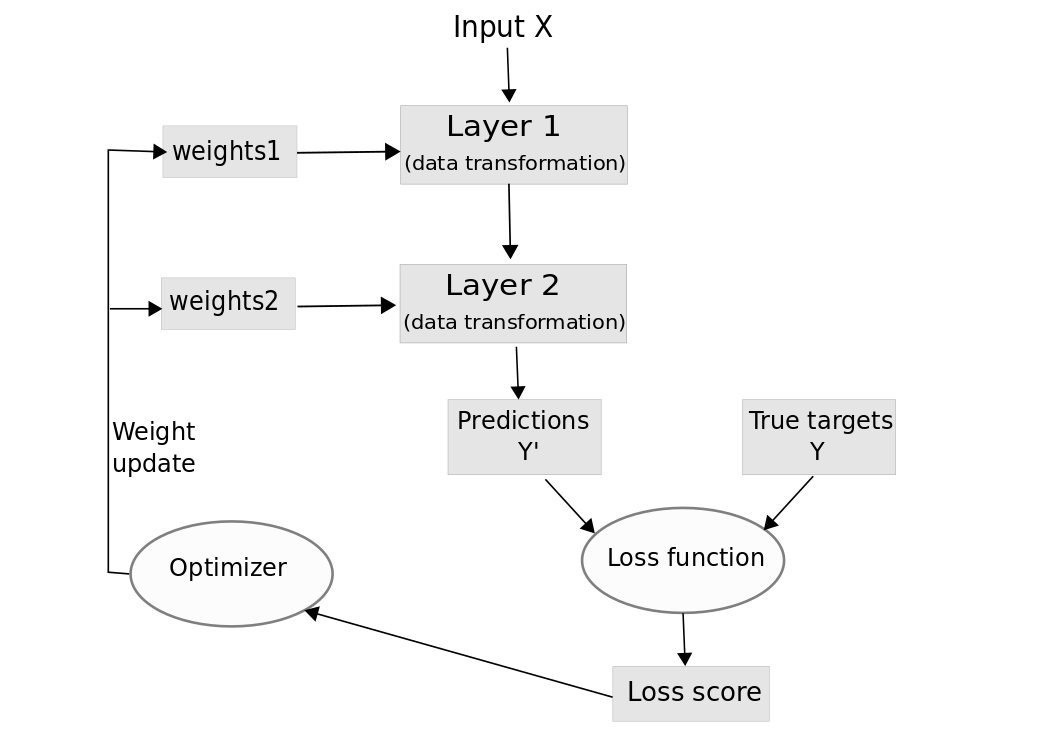
\includegraphics[width=12cm,height=10cm,keepaspectratio]{images/deep_learning_basics.png}
		\caption{Building block of deep learning process }
		\label{fig:deep learning architecture}
	\end{center}
\end{figure}

\subsection{Why data augmentation?}

Deep learning requires a relatively large amount of data and significant computing power to analyze the data. Furthermore, it  requires an efficient algorithm that can calculate hundreds of weights. These requirements posed by deep learning were the significant barriers to the application of deep learning in early 90's. However, nowadays there has been a substantial improvement concerning Central Processing Unit (CPU) and Graphical Processing Unit (GPU). Similarly, digitalization and increasing reach of the internet has generated a significant amount of data. In addition, open source projects contributed by both corporations and researchers in the field of deep learning has streamlined the implementation and deployment of deep learning. As a result of all this, deep learning has been applied to solve various complex problems like image and speech recognition, analyzing particle accelerator data, DNA mutations and autonomous driving with successful results \citep{lecun2015deep}. 

Empirical studies have shown that data representation obtained from deep learning often yield better machine learning results in terms of improved classification modeling \citep{larochelle2009exploring}. Similarly, data generated by a deep learning model is also deemed to be of a better quality than the data generated by generative probabilistic models \citep{najafabadi2015deep}. Compared to conventional machine learning techniques, deep learning technique offers better performance and makes problem-solving simpler by requiring less data engineering and domain expertise. Deep learning is able to capture relevant features of complex problems with the help of multiple representations. Deep learning is simple, scalable, versatile and reusable. It is simple in a sense that it does not require feature engineering which means it removes complex machine learning pipelines with a simple end-to-end trainable models. Thanks to various open source projects, deep learning computation can be parallelized on GPU's or in a distributed system. Deep learning models are trained by iterating over a small batch of data. This batch processing adds the flexibility to train on any size of data. Furthermore, deep learning models are modular allowing the layers from model to be reused to solve similar problems. These pragmatic properties make deep learning functional and useful for researchers and companies alike.    

\section{Data Augmentation in Deep Learning}
Data augmentation has been applied in deep learning with varying degrees of success. The most prominent application of data augmentation has been in image classification, and it has proven to be a successful technique to improve the accuracy of a model \citep{krizhevsky2012imagenet}. Data augmentation can reduce over-fitting as well as make model more robust by introducing artificially generated variables that make the training sample diverse. For example, a recent study on the application of data augmentation in facial recognition showed a significant improvement in the model as a result of data augmentation \citep{kortylewski2018training}. This thesis will primarily go through three data augmentation methods, namely data warping, synthetic minority over-sampling technique, and generative adversarial nets. 

\subsection{Data Warping} 
The most conventional application of data augmentation has been in image classification, and it has proven to be reasonably successful to improve the accuracy of a model. One of the widely used and accepted practices for augmenting image data is to perform geometric and color transformation, such as reflecting an image, cropping and translating the image. Through the application of the various transformation to one image, multiple images can be generated with different perspective and shades. These newly generated images can be used as new training samples. This approach of data augmentation is known as data warping. The term data warping was first used in the context of producing random variations in hand-printed English text data so that new characters are generated mimicking the stylistic variation within and between the writers \citep{yaeger1997effective}.

From its initial application in late 1990 this technique was further extended to improve the performance of a neural network and achieve record performance of the time on MNIST handwritten digit database using a neural network in 2003 \citep{wong2016understanding}. Training data was created by applying simple distortion such as translations, rotation, and skewing. These various transformations helped to create naturally occurring variation as different individuals write letters slightly differently. Augmenting data through the techniques of data warping depends on the problem at hand. Furthermore, these techniques are heuristic in nature which is not guaranteed to be optimal in all situations.

\begin{figure}[ht]
	\begin{center}
		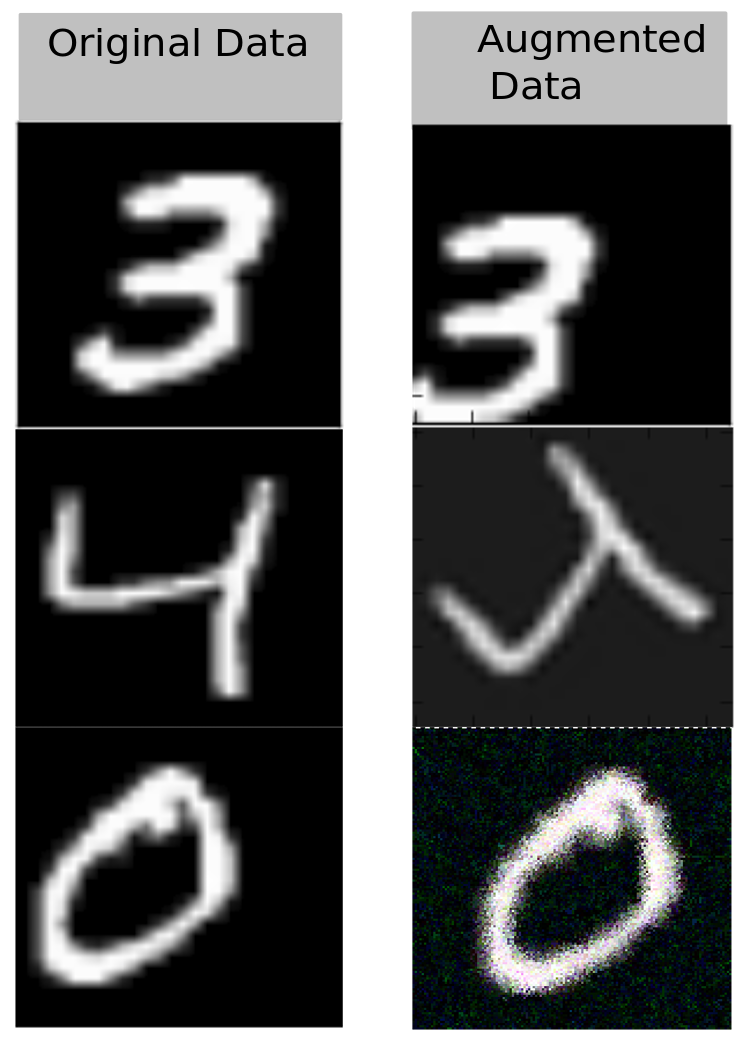
\includegraphics[width=12cm,height=10cm,keepaspectratio]{images/simple_augment_mnist.png}
		\caption{Augmentation via data warping on hand written digits}
		\label{fig:data warping}
	\end{center}
\end{figure} 

The figure ~\ref{fig:data warping} shows the data augmentation applied to image data using various data warping techniques. The top image is warped using a simple random shift of pixels, whereas the bottom image of zero is warped by adding random noise to pixels, and the middle image of four is warped using just a rotation of pixels. This simple technique can make the model more robust. For example by artificially generating several many variation of hand written digit, model can capture naturally occurring variation in hand-writings. This analogy can be extended to the spectral data also, as they can shift slightly up or down due to the variation in concentration or due environmental factors compared to the sample prepared in the lab. Thus, by training model with augmented data model is likely to generalize well in previously unseen measurement data. 

\subsection{SMOTE}
Synthetic Minority Over-Sampling Technique (SMOTE) is a data augmentation technique which is inspired by data warping, particularly its ability to reduce the class imbalance in hand-written digit problems \citep{chawla2002smote}. It is a data augmentation approach in which minority label is over-sampled by creating new synthetic data. This method has been used mainly to address the problem of class imbalance, where real-world data-sets often contain a small percentage of target class examples. The advantage of SMOTE compared to data warping is that synthetic samples are generated in feature space, and this property of SMOTE algorithm makes it application-independent \citep{chawla2002smote}. 

New synthetic samples are obtained from the minority class using the information available in the data. Synthetic samples are generated by taking the difference between feature vector under consideration and its nearest neighbor, then multiplying this difference by a random number between 0 and 1 and finally adding it to the feature vector under consideration \citep{chawla2002smote}. For each sample $x$, the other samples from the same minority class with the smallest Euclidean distance from the $x$ are identified. These other samples are also called as nearest neighbor. One of the nearest neighbors is randomly picked $x^{R}$. The new synthetic sample $S$ is defined in the equation below.

\begin{equation}
S= x + u(x^R -x), where\ u \sim U(0,1) 
% S = x + u.(x^R-x), u ~ U(0,1)
\end{equation} \citep{chawla2002smote} 

Figure ~\ref{fig:SMOTE} succinctly summarizes the synthetic data generation process using SMOTE.

\begin{figure}[ht]
	\begin{center}
		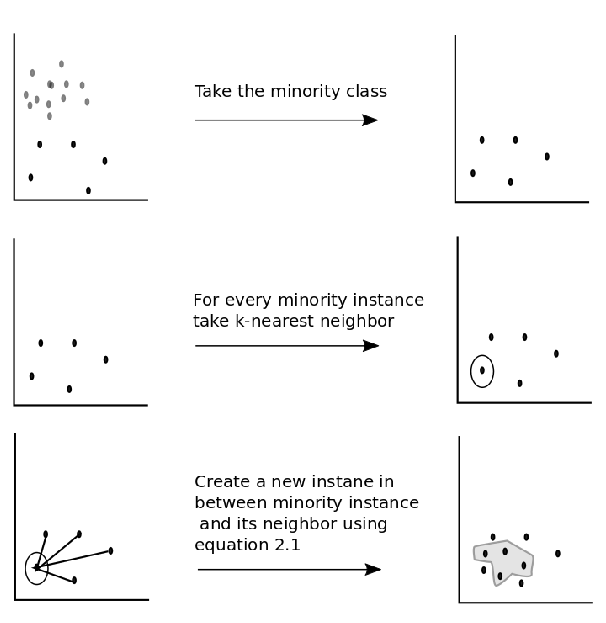
\includegraphics[width=12cm,height=10cm,keepaspectratio]{images/SMOTE_2.png}
		\caption{Synthetic data generation using SMOTE}
		\label{fig:SMOTE}
	\end{center}
\end{figure} 

One alternative to SMOTE is to over-sample the minority class with replacement. Some previous study has shown that while this practice can increase the number of samples in training set, it does not significantly increase the class recognition of minority class \citep{chawla2002smote}. In the experiment conducted by \citet{chawla2002smote}; when the minority class was over-sampled by increasing amounts, the decision tree tried to identify similar but more specific regions in the feature space of minority class. In other words, the replication of same data causes the model to focus on those repeated samples and also to over-fit the data. Over-sampling the minority class with replacement can produce an undesired result of shrinking the decision boundary for minority class. Ideally, we would want to increase the decision boundary of minority class so that it generalizes well for unseen data. In the same paper, \citet{chawla2002smote} demonstrated that SMOTE approach could improve the accuracy of the classifier for a minority class by applying it on various imbalanced data-sets.

\subsection{Generative Adversarial Nets}
One of the promising techniques of data augmentation in the field of deep learning is Generative Adversarial Nets (GANs). It is a powerful technique to generate data. GANs uses a min-max strategy where one neural net successively generates counterfeit samples from the original data distribution in order to fool the other net, and the other net is then trained to better distinguish the counterfeits \citep{goodfellow2014generative}. There are two main elements of a GANs: Generator and Discriminator. The objective of the generator is to take a random input and generate a sample data, whereas the objective of the discriminator is to take input from the original data or data generated from generator and to predict whether the input is real or generated. Discriminator aims to maximize the probability of assigning the correct label to both original sample and the counterfeit, whereas generator simultaneously aims to minimize the difference between original and counterfeit samples \citep{goodfellow2014generative}. In this sense, the discriminator and generator play a two-player mini-max game. The generator obtained from this process can be used to generate synthetic samples of data which closely represents the actual data. The figure below illustrates the GANs architecture.

\begin{figure}[ht]
	\begin{center}
		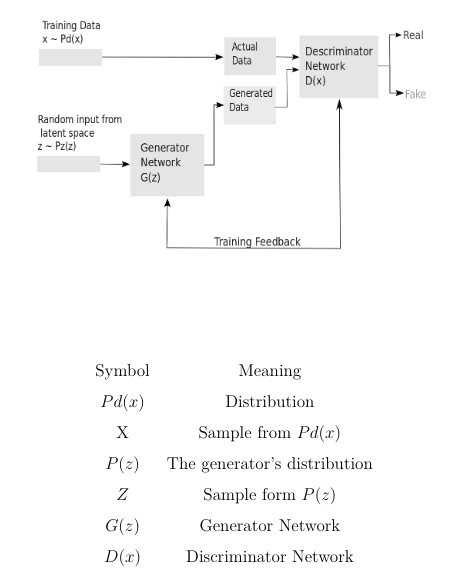
\includegraphics[width=12cm,height=13cm,keepaspectratio]{images/GAN_3.png}
		\caption{GANs architecture}
		\label{fig:GAN}
	\end{center}
\end{figure} 

%\begin{center}
%	\begin{tabular}{ c c }
%		Symbol & Meaning  \\ 
%		$Pd(x)$ & Distribution \\ 
%		X & Sample from $Pd(x)$  \\  
%		$P(z)$ & The generator's distribution \\  
%		$Z$ & Sample from $P(z)$ \\      
%		$G(z)$ & Generator Network \\  
%		$D(x)$ & Discriminator Network 
%		
%	\end{tabular}\\
%\end{center}


Here, generator $G(z)$ takes an input from $P(z)$. The generated data is supplied to discriminator network along with the actual data. The discriminator takes input $x$ from $Pd(x)$ where $Pd(x)$ is the real distribution, $D(x)$ then solves a binary classification problem. Two models compete against each other which ideally leads to the generator being able to produce fairly real looking samples from $P(z)$. This process can be mathematically represented as:

\begin{equation}
min_{G}max_{D}L(D,G) = E_{x \sim Pdata(x)}[logD(x)]+E_{z \sim P_{z}(z)}[log(1-D(G(z)))]
\end{equation} 
\citep{goodfellow2014generative}

In equation 2.2 first term is entropy that the data from real distribution $P_d$ passes through the discriminator. We want to maximize discriminator given real data $P_{d}(x)$ by maximizing $E_{x_{d}(x)}[logD(x)]$. Meanwhile given fake data $P_{(z)}$ the discriminator is expected to output a probability of $D(G(z))$ close to zero by maximizing second part of equation $E_{z~P_{z}(z)}[log(1-D(G(z)))$. Whereas, the generator is trained to increase the chances of $D(x)$ producing a high probability for a fake example, thus to minimize $E_{z~P_{z}(z)}[log(1-D(G(z)))$.

GANs has been extensively used in machine learning applications such as computer vision and image recognition. GANs have been useful even with relatively small sets of data as one can use a transfer learning technique. GANs have been used for example to train a self-driving car to drive in the night or rain using only data collected on a sunny day \citep{gurumurthy2017deligan}. Recently there have been many studies in the application of GANs in medical diagnosis mainly to augment the medical imaging data. Medical industry also faces the problem of limited data, as data is heavily regulated and costly to acquire. In one recent study conducted by \citet{frid2018synthetic}, authors successfully used GANs to augment the limited medical image data to improve a deep learning model. Using GANs as augmentation method authors were able to gain 7 percent improvement in accuracy over the traditional augmentation methods like data warping. 

GANs offer a unique proposition in data augmentation. Unlike data warping, instead of figuring out augmentation that is label invariant we let the deep learning model to find the label invariant augmentation. Thus, the expectation from the GANs model is that the data is generated from the actual data distribution so that the newly generated data has the core characteristics of real data.   

\section{Model Evaluation}

Since the thesis tries to evaluate the performance of various deep learning models, metrics for model assessments needs to be clearly laid out. Model evaluation depends on the type of problem model is trying to solve. Machine learning divides classification problem into binary, multi-class, multi-labeled and hierarchical tasks \citep{sokolova2009systematic}. The classification problem tackled in this thesis falls under the multi-class classification problem. Formally multi-class problem is defined as a classification problem where the input is to be classified into one and only one, of 'l' non-overlapping classes \citep{sokolova2009systematic}.

Empirical evaluation remains the most used approach for the model assessment \citep{sokolova2009systematic}. The empirical comparison is made through applying algorithms from the model on data-sets that are not used for model training and then evaluating the performance of the classifiers that the algorithms have produced. Often accuracy remains the most used evaluation measure for evaluating models \citep{sokolova2009systematic}. However, accuracy is not the only measure for performance evaluation. The performance of a classification algorithm from given model can also be evaluated by dividing the accuracy into smaller components. For instance, computing the number of correctly recognized class examples (true positives), the number of correctly recognized examples that do not belong to the class (true negatives), and examples that either were incorrectly assigned to the class (false positives) or that were not recognized as class examples (false negatives) \citep{sokolova2009systematic}. These four values constitute a confusion matrix shown in the table ~\ref{table:Confusion matrix}.



\begin{table}[ht]
	\centering
	\caption{Confusion matrix for binary classification }
	% Place the label just after the caption to make the link work
	\label{table:Confusion matrix}
	\begin{tabular}{|p{3cm}|p{4cm}|p{4cm}|} 
		% Alignment of sells: l=left, c=center, r=right. 
		% If you want wrapping lines, use p{width} exact cell widths.
		% If you want vertical lines between columns, write | above between the letters
		% Horizontal lines are generated with the \hline command:
		\hline
		\textbf{Data class} & \textbf{Classified as pos}& \textbf{Classified as neg}\\ 
		\hline % The line on top of the table
		\textbf{pos} & true positive (tp) & false negative (fn) \\ 
		\textbf{neg} & false positive (fp) & true negative (tn)  \\ 
		
		% Place a & between the columns
		% In the end of the line, use two backslashes \\ to break the line,
		% then place a \hline to make a horizontal line below the row 
		
		\hline		
	\end{tabular} % for really simple tables, you can just use tabular
	% You can place the caption either below (like here) or above the table
	
\end{table} % table makes


Accuracy is just a proportion of the total number of prediction that was correct. Precision and recall provided more insight than just the overall accuracy. To use the analogy of cancer diagnosis problem: precision tells what proportion of patients diagnosed by the model as having cancer had cancer whereas recall tells what proportion of patient that actually had cancer was diagnosed by the model as having cancer. What precision and recall do is they break the accuracy into small metrics like true positive, false positive and false negative. Precision is defined as the number of true positives over the number of true positives plus the number of false positives. Recall is defined as the number of true positives over the number of true positives plus the number of false negatives \citep{scikit-learn}. Furthermore, often precision and recall are expressed in one number which is its weighted average known as the F1 score. In other words F1 score is just the harmonic mean of precision and recall.

\begin{equation}Accuracy = \dfrac{TP + TN}{TP+TN+FP+FN}\end{equation} 
\begin{equation}Precision = \dfrac{TP}{TP+FP}\end{equation} 
\begin{equation}Recall = \dfrac{TP}{TP+FN}\end{equation} 
\begin{equation}F1 = \dfrac{2 (recall \times precision) }{recall+precision}\end{equation} 

The above metrics are expressly designed for the binary classification task, where the input is to be classified into one, and only one, of two non-overlapping classes \citep{sokolova2009systematic}. However, these binary metrics can be easily extended to the multi-class problem. There is a number of ways to average binary metric calculations across the set of classes. One way to averaging binary metric is macro averaging. Macro averaging calculates the mean of the binary metrics, giving equal weight to each class. In problems where infrequent classes are important, macro-averaging can be a means of highlighting their performance \citep{scikit-learn}.

\begin{equation}Precision_M =  \dfrac{\sum^l_i\dfrac{tp_i}{tp_i+fp_i}}{l} \end{equation} 
\begin{equation}Recall_M =  \dfrac{\sum^l_i\dfrac{tp_i}{tp_i+fn_i}}{l} \end{equation} 
\begin{equation}Fscore_M =  \dfrac{2 (Precision_M \times Recall_M) }{Precision_M+Recall_M }\end{equation}

To summarize, there are various metrics for evaluation of classification models. For a multi-class classification problem, model metrics are merely the extension from binary classification metrics. It is often the case that no single metrics can comprehensively measure and evaluate the quality of the model. Therefore depending on the application of model, relevant application metrics needs to be used. In this thesis, macro-averaging is used to evaluate the models, as this approach will emphasize the quality of the model based not only on the accuracy of majority class but also based on infrequent minority classes.



%\startchapright\input{3environment.tex}

\startchapright\chapter{Methods}
\label{chapter:methods}

\section{Cross Industry Standard of Data Mining}
Data mining is a process of knowledge extraction or information discovery from a large number of data \citep{kurgan2006survey}. In this sense, one can argue that data mining is a blanket term for all kind of knowledge discovery processes including machine learning. For data mining to work, several technologies and techniques need to work together. Data mining incorporates various techniques and technologies like database management, computing infrastructure, statistical methods, data visualization, and communication. In order to successfully carry out knowledge discovery process one needs effective standards for various aspects of data mining.
 
Conceived by the consortium of multinational companies, Cross-Industry Standard of Data Mining (CRISP-DM) encapsulates a tried and tested method for data mining that builds upon previous attempts to define knowledge discovery methodologies. Although it is a somewhat old process conceived in 1996, the iterative process outlined in a CRISP-DM is still pragmatic in contemporary data science projects. Apart from being an iterative data-driven process, CRISP-DM also links the business understanding and objectives to data science projects. The inclusion of a business aspect to data mining adds a more nuanced business perspective to data science projects. CRISP-DM is one of the most popular and broadly adopted data mining models which has been acknowledged and relatively widely used in both research and industrial communities \citep{kurgan2006survey}. The figure~\ref{fig:Crisp process} below summarized the iterative process of CRISP-DM.

\begin{figure}[ht]
	\begin{center}
		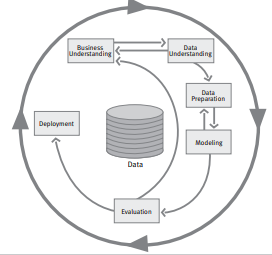
\includegraphics[width=7cm,height=7cm,keepaspectratio]{images/new_crisp.png}
		\caption{CRISP-DM process}
		\label{fig:Crisp process}
	\end{center}
\end{figure} 

CRISP-DM is a comprehensive process that starts with business understanding and ends with the final deployment of a data mining solution. Therefore it has various sub-steps within its main six phases. This thesis does not strictly follow the entire process because the primary objective of the thesis is not necessarily to obtain and deploy a production-level model but to find a way to improve the existing model with the help of data augmentation. Therefore, CRISP-DM is used as the reference model for developing and evaluating various machine learning algorithms built in the thesis.

\subsection{Business understanding}
All data science projects are a means to an end, the end usually being the business objective. To successfully carry out the data science project, a clear understanding of the underlying business objective is vital. So in this phase, the prime focus is on understanding the project objectives and requirements from a business perspective, then converting this knowledge into a data mining problem definition and data mining objective \citep{chapman2000crisp}. 

\subsection{Data understanding}
After understanding the business goal and setting the data mining objective next logical step is to collect and analyze the relevant data. This stage primarily deals with querying data from the database and checking whether the data is fit to carry out data mining process. Similarly, the first general insights are also discovered during this phase which helps to enhance the understanding of data at hand.

\subsection{Data preparation} 
Data in its raw-form cannot directly be used for modeling. Data needs to go through some preparatory steps.
Therefore this phase includes various activities undertaken to construct final data-set which will be fed into machine learning models. The first step often will be to clean the data, meaning remove the data that is corrupted, missing or unnecessary. Then if needed perform transformation such as normalization. This is also a phase where various augmentation techniques are applied to get the final data that is fed to the deep learning model.

\subsection{Modeling} 
This phase involves selecting the appropriate machine learning model which can achieve the goal outlined in the initial phase. Usually, various methods can be used to achieve the same goal. For example, one can use various machine learning strategies for classification task from simple logistic regression to convolutional neural network. Thus, different methods can be tested to determine the optimal method. This phase also includes designing testing set and some initial assessment of the model.

\subsection{Evaluation}
Once the modeling is completed models need to be evaluated. Before proceeding to deployment, the model needs to be thoroughly evaluated to make sure that it achieves the business objective and needs. Model evaluation can take several forms such as simple analysis of the accuracy of model's prediction on evaluation data, analyzing the complexities of the algorithm to the speed at which model takes time to execute. There is no one silver bullet for model evaluation as there are a variety of evaluation measures depending on the business objective and need. Thus, a model needs to evaluated based on the measure that most accurately reflects the business needs.

In this thesis, an entire chapter has been devoted to model evaluation as one of the crucial tasks of the thesis is to evaluate various machine learning models obtained through various augmentation techniques.   

\subsection{Deployment}
Once the suitable model meeting business needs is created, it needs to be deployed in the field. Depending on the objective of business it could be from as complicated as deploying machine learning model in a distributed cloud environment to as simple as generating a simple report for communicating and implementing the insights gathered from data mining process. Since model deployment is out of the scope of the thesis, it will not be discussed in subsequent chapters. 
 
 


 
\startchapright\chapter{Implementation}
\label{chapter:implementation}

This section outlines the application of data mining process. In this thesis python programming language is used to implement various data augmentation as well as to build deep learning model. Deep learning is implemented using Keras. ``Keras is a high-level neural network API written in Python and is capable of running on top of TensorFlow, CNTK or Theano''-- \citep{chollet2015keras}.  

\section{Business understanding}
As outlined in the motivation section, case company manufactures the portable near-infrared spectrometer. Near-infrared spectroscopy(NIRs) can measure the chemical composition of biological materials by analyzing the diffuse reflectance or transmittance of the samples at several wavelengths from 700 to 2500 nanometers. One of the unique properties of infrared spectrum is that no two organic compounds have the same infrared spectrum \citep{rsc}. Pure compounds can be identified by examination of their spectra provided that a chemist has a copy of the spectrum so any unknown pure compound can be identified by making a comparison \citep{rsc}. This process is straightforward in theory, however in practice due to sample variation, environmental factors and device variations, spectra from two same compounds might not necessarily be identified by making a simple comparison. That is why a machine learning model is needed which takes into consideration several factors and can identify compound based on previously trained data.

NIRs has been widely used in various food commodities especially in the grain, cereal products, and oil-seed processing industries \citep{elmessery2014manufacture}. It is also extensively used in chemical and pharmaceutical industries for classification of raw materials \citep{elmessery2014manufacture}. NIRs technology is gaining popularity for material detection as it is fast, reliable, non-destructive, and relatively cheaper \citep{evans1999near}. Furthermore, there is very minimal sample preparation, or pretreatment and material are preserved after the examination. Therefore NIRs solution provides various advantages over the other types of material sensing solutions.

One of the major hindrances for the application of NIRs has been the size and cost. Conventional spectrometers are relatively big and are also costly. However, the spectrometers produced by the case company are portable and economical. As discussed above, portability adds some complexities, however the advantages over-weight the drawbacks. The portability offers a novel application of NIRs solution in various mass markets, not just limited to traditional agricultural and pharmaceutical industries. 

Overall innovative NIRs solution offered by the case company has significant potential and offers quite many advantages over a traditional sensor. Despite its advantage, there are also several challenges. Traditionally the measurement with the spectrometer is carried out in a controlled environment in a laboratory setting where the environmental variables such as temperature, lights and moisture level can be controlled, enabling consistent measurements. Due to the portable nature of the product, above mentioned environmental variables cannot be controlled. The fluctuation in environmental variables introduces fluctuation in a measurement. The fluctuation of measurement means that the classifier needs to be trained in a diverse sample of data, mimicking the actual use condition. Similarly, samples in the real world come from various sources with a various level of concentration. At present companies try to capture all the environmental as well as sample variation in a laboratory to produce training samples. However, there are several variations, and this takes a considerable amount of time to produce data to train a deep learning model. Similarly, due to regulatory restriction pharmaceutical materials are not readily available, restricting the pool of available samples to train a deep learning model. Furthermore, due to the nature of the manufacturing process, no two scanners are the same. So this means there will be slight variation in a measurement of the same sample from two different scanners. Therefore there is a need for robust model that can take various factors in consideration and correctly classify materials. 

The primary business objective is to produce a robust model that can classify material from the measurement data produced from the portable spectrometer with reasonable accuracy despite all the challenges discussed above. The aim is also to reduce the data acquisition cost and time. To achieve this business goal, data augmentation with deep learning is deemed to be the suitable tool, as data augmentation has the potential to save both time and money in data collection and also improve the generalization ability of the model by increasing the diversity of samples. As mentioned above, there is a precedence of data augmentation being used in a similar situation with a successful result.  

\section{Data understanding}
The primary source of data analyzed in this thesis comes from the NIR spectrometer. A spectrometer analyses a compound by passing near-infrared radiation over a range of different frequencies and measuring the absorption made by each type of bond in a compound. This produces a spectrum, usually a plot of percent transmittance against wave-number. In simple words, transmittance describes how much light passes through a sample unchanged and is measured as a percentage. The image illustrated in figure ~\ref{fig:Spectral data} below illustrates the typical data obtained from spectrometer which is a plot of percent transmittance against wave-number.

\begin{figure}[ht]
	\begin{center}
		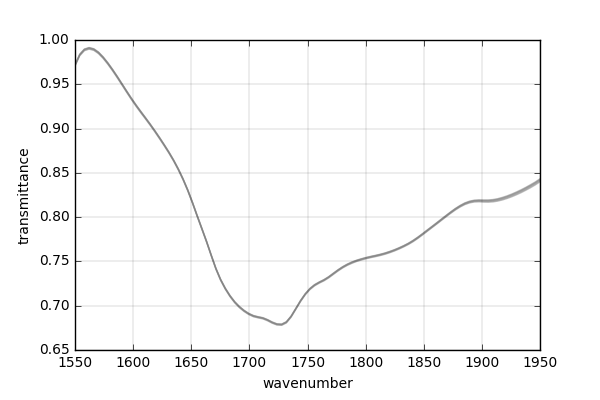
\includegraphics[width=\textwidth]{images/spectral_graph.png}
		\caption{Spectral data}
		\label{fig:Spectral data}
	\end{center}
\end{figure}


As discussed above NIRs is used extensively in pharmaceutical industry to detect raw materials. Incidentally, pharmaceutical raw materials are also among the most heavily regulated materials, so there is limited sample available for training a neural network. As a result, pharmaceutical raw materials are ideal for testing effectiveness of data augmentation. The model built in the thesis will try to detect four different pharmaceutical raw materials. These four different pharmaceutical compounds will be called as variables '0',1','2','3' and '4' respectively. These variables are coded as a categorical variable with label '0','1','2','3' and '4'. The compound '0','1','2' and '3' are hard to acquire. Label '4' constitute the compounds that are readily available, and therefore this label is the majority class.

\subsection{Exploratory Analysis}
Pharmaceutical compounds '0', '1','2' and '3' are closely related to each other but are not the same compound. Whereas the compound '4' contains several different compounds that do not belong to any '0','1','2' and '3'. The target variables are not 100 percent pure compound. The concentration of the target varies anywhere from 5 to 100 percent. Figure ~\ref{fig:variable concentration} shows the concentration count for all the compound.

\begin{figure}[ht]
	\begin{center}
		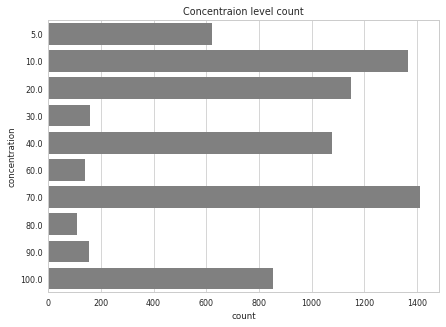
\includegraphics[width=\textwidth]{images/variable_composition.png}
		\caption{Concentration level of compounds}
		\label{fig:variable concentration}
	\end{center}
\end{figure}

As we can see from the figure ~\ref{fig:variable concentration} concentration varies quite a lot. Most compounds have the concentration of 70 percent followed by the 10 percent. Not many compounds have the concentration level of 80 percent. The concentrations of unknown samples are unknown and therefore are not shown in the figure~\ref{fig:variable concentration}. The task of the classifier is to detect the compound regardless of the concentration. Given the spectral data, the classifier has to detect whether there is a presence of target compound or not irrespective of its concentration level. 

\section{Data preparation}

 Spectral data is collected from the spectrometer and stored in a central database. The data does not need extensive data preparation as it is reasonably clean with some exception of missing labels. To prepare the data, samples with missing labels are removed, and the data is transformed using a couple of domain-specific data transformations such as Fourier transformation. Fourier transformation takes a signal and expresses it in terms of the frequencies of the waves that make up that signal. These transformations enable us to compress the data to 50 points from 100 points of spectra.

As discussed earlier, data preparation phase included all the steps undertaken to create a final data-set that is fed to the deep learning model. Consequently, data augmentation is a part of this phase. Above mentioned augmentation techniques, namely data warping, SMOTE, and GANs, will be implemented in the following sub-section.

\subsection{Data augmentation using data warping}
Data warping is one of the simplest and easiest ways to apply data augmentation. In a prominent neural network implementation library Keras, data augmentation for images such as transformation, scaling, rotation and other similar transformations are natively supported. As described earlier, data warping creates new data primarily using a transformation that rotates, shifts or adds distortion which still preserves the label. This type of augmentation for image data is quite straightforward as these types of transformations preserve the image label. For example, rotated image data of a cat still retains its label as cat image upside down is still a cat image. However, for spectral data, augmenting the data by rotation no longer preserves the label. In this sense augmenting data using the data warping technique is highly domain specific and requires a thorough understanding of data at hand.

For spectral data, the appropriate augmentation was to add a small amount of randomly distributed slope so that the points are slightly shifted up or down from the original data. By adding a small amount of slope, we assumed that it could mimic the variation caused by measuring the same sample under different conditions such as humidity, temperature and sample concentration. The figure below illustrates the augmentation on the spectral data along with the similar augmentation on image data. The simple algorithm used to augment data is presented in appendix~\ref{chapter:first-appendix}.

\begin{figure}[ht]
	\begin{center}
		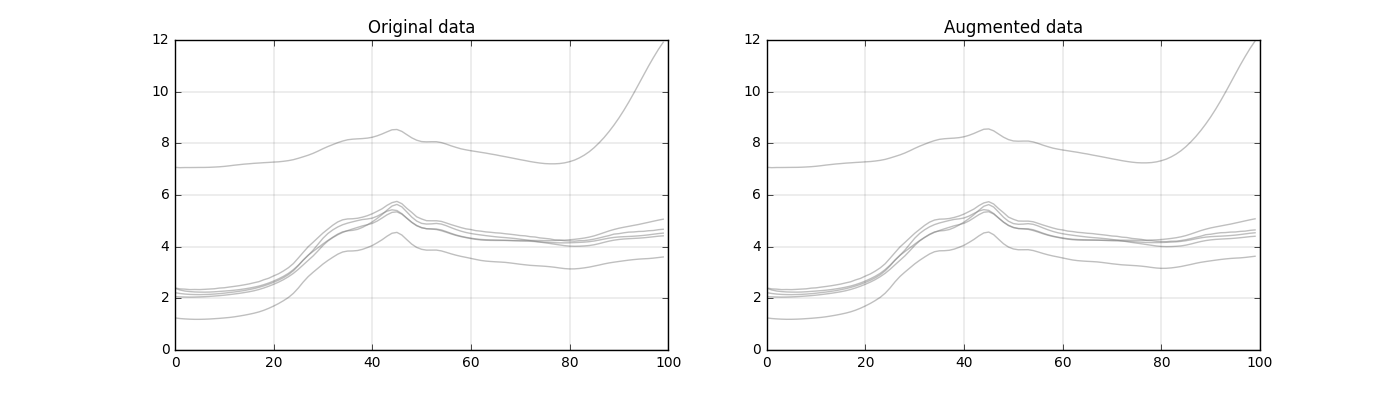
\includegraphics[width=\textwidth]{images/simple_augment.png}
		\caption{Augmentation using data warping}
		\label{fig:simple augmentation}
	\end{center}
\end{figure}


The random points added to the original point is minimal, therefore augmented data is not easily differentiable from the original. However, on close observation, we can observe that augmented data have points slightly up or down compared to the original figure. This type of data augmentation is akin to distorting the image by adding random noise. Depending upon the augmentation the value of noise can be increased or decreased by adjusting the parameters from where the random noise is generated. 

\subsection{Data augmentation using SMOTE} 
SMOTE was conceived to better handle the imbalance data-sets by oversampling the minority class. What SMOTE does is it leaves the majority class intact, in this case unknown samples, and it creates synthetic samples for all other minority classes so that all the class labels are represented equally in the final data set. The details of how SMOTE is implemented is already discussed in the theoretical review section. The augmentation using SMOTE was implemented via python module called 'imblearn' \citep{JMLR:v18:16-365}. This implementation is displayed in appendix~\ref{chapter:second-appendix}. Figure ~\ref{fig:SMOTE augmentation} shows the generated synthetic samples from SMOTE. 


\begin{figure}[ht]
	\begin{center}
		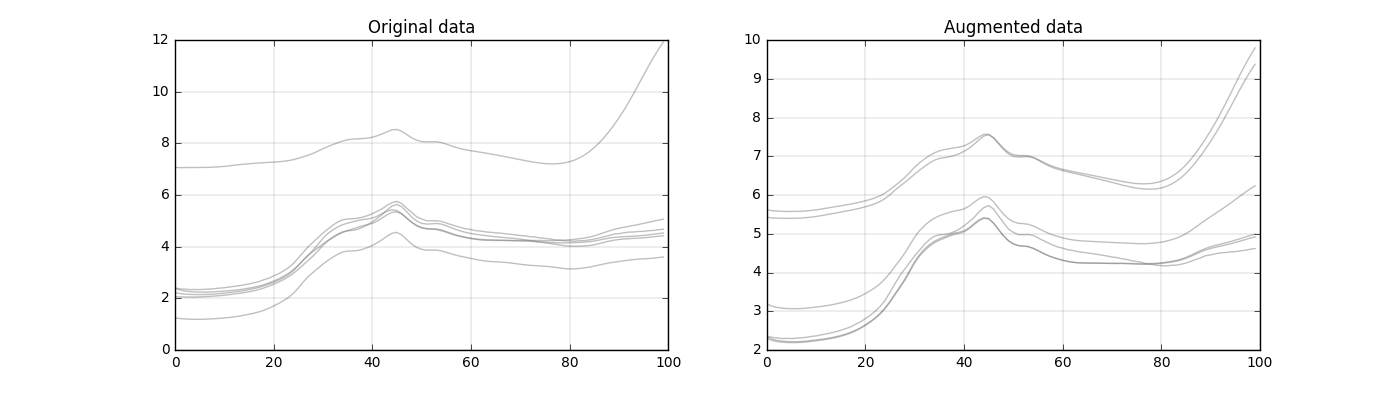
\includegraphics[width=\textwidth]{images/smote_augment.png}
		\caption{Augmentation using SMOTE}
		\label{fig:SMOTE augmentation}
	\end{center}
\end{figure}

In the figure~\ref{fig:SMOTE augmentation} we can see that augmented data have a bit more variation than the augmented data through data warping. The new generated spectral data is just an interpolation of new data between existing data. As we can observe from the figure~\ref{fig:SMOTE augmentation} original y value is within the range of 1 to 12, and the augmented data y value is also within that same range. One can argue that this behavior is ideal because in a field setting the spectrometer measurement can fluctuate within the range of training samples.  

The overall idea of augmentation in SMOTE is quite similar to data warping. The augmented data is merely shifted up or down. However, in data warping the data was created simply by adding random points to one spectral data. Here the data is interpolated between a spectral data and its k-nearest neighbor. This technique increases the variation of the sample compared to data warping.   
 
\subsection{Data augmentation using GANs}
To implement the GANs laid out in the literature review we make two deep learning models: one generator and another discriminator. Then we stack together the two models and start a model training process. The architecture of the GANs model is illustrated in the figure below.

\begin{figure}[ht]
	\begin{center}
		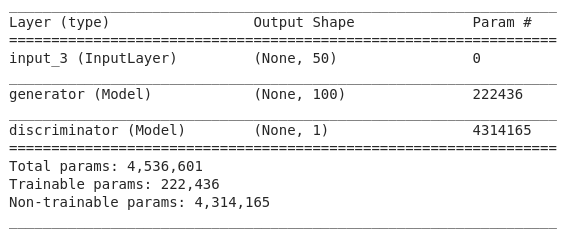
\includegraphics[width=\textwidth]{images/GAN_architecture.png}
		\caption{The implementation of GAN in keras}
		\label{fig:GAN architecture}
	\end{center}
\end{figure}

Here the generator model turns a vector that is randomly sampled from normal distribution into a data mimicking the actual data generated from the sensor. One common problem with GANs is sometimes generator gets stuck with generating data that is just noise. A possible solution is to use a dropout layer on both the discriminator and the generator. Here the discriminator model takes as input a data that is generated or actual and classifies it into one of two classes: ``generated data''  or  ``real data''.

The figure~\ref{fig:GAN architecture} shows a GANs network architecture in Keras interface. In GANs architecture two models, discriminator and generator, are chained together into GANs network. When trained, the model will move the generator in a direction that improves its ability to fool the discriminator. Generator and discriminator are just two neural networks.

The first step of the training process is to draw random points from the normal distribution, and then generate a data from those random points. The second step is to mix the generated data with actual data, then label it either ``real'' or ``generated'' and feed it into the discriminator. The third step is to draw new random points from a normal distribution and train GANs using these random vectors, which are all labelled as ``real''. This third step effectively updates the weights of the generator to move them toward getting the discriminator to predict ``real'' for generated data \citep{chollet2017deep}. The figure~\ref{fig:GANs augmentation} shows the generated images from the GANs. From the figure~\ref{fig:GANs augmentation} we can see that augmentation from GANs is unlike any other before. The other augmentation strategies closely replicated the actual shape of original data, whereas generated data from GANs do not have smooth slopes like original data. The full implementation using python and Keras is illustrated in appendix~\ref{chapter:third-appendix}.


\begin{figure}[ht]
	\begin{center}
		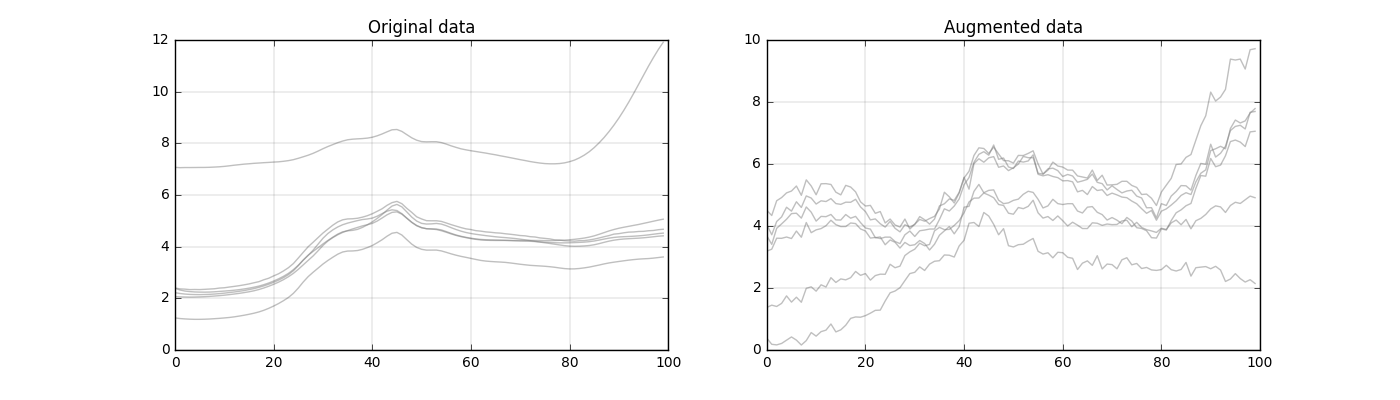
\includegraphics[width=\textwidth]{images/gan_augment.png}
		\caption{Augmentation using GANs}
		\label{fig:GANs augmentation}
	\end{center}
\end{figure}

\section{Modeling}
In this phase, we build deep learning models using data prepared through different augmentation methods. A neural network was chosen primarily because of its ability to handle high dimensional data, the requirement of little feature engineering and the availability of open source libraries that can leverage graphical processor for a speedy result. There are various types of neural networks, and in this thesis, we will be working with the kind of network known as the convolutional neural network.

Convolutional neural network was chosen primarily because unlike the typical dense layers, convolution layers learn local patterns in their input feature space whereas dense layers learn global patterns \citep{chollet2017deep}. Furthermore, convolution net can learn the spatial hierarchies of patterns. These critical characteristics of convolution net makes it translation invariant, meaning that the convolution net can recognize the patterns, no matter where they are. \citep{chollet2017deep}. For example, convolution network is quite successful in image classification because it can detect the local patterns along with its spatial hierarchies such as eye, nose and mouth, no matter where they are located in the image. Since we are treating the data obtained from spectrometer as a fingerprint of the particular chemical compound, identifying local patterns and hierarchies in spectral data can help in accurately classifying one fingerprint from another. The figure~\ref{fig:Convolution model} illustrates the architecture of the convolution neural network used for modeling. 

The model was trained for 30 epochs in mini-batches of 2000 samples. Epoch means merely the number of iteration over all the samples in training data, whereas batch is the number of training data that is used to update the weights. We do not pass the entire data set into the neural network at once but instead divide the data into a number of small batches. On completion of every batch, the loss is computed, and weights of networks get updated.


\begin{figure}[ht]
	\begin{center}
		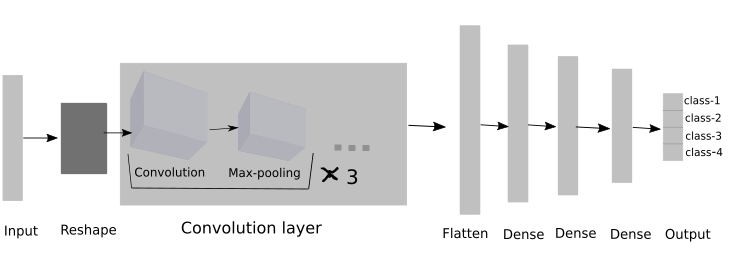
\includegraphics[width=\textwidth]{images/neural.png}
		\caption{Model Architecture}
		\label{fig:Convolution model}
	\end{center}
\end{figure}

Picking the right network architecture is more of an art than a science-- \citep{chollet2017deep}. Having said that, there are some best practices and generally accepted conventions. The architecture of network proposed in the thesis is based on the best practices and generally agreed principles. For instance, categorical cross-entropy is used as the objective function of the model, as it is generally used for multi-class classification problems. Similarly, convolutional layers are followed by a max-pooling layer which is also a common practice in designing convolutional network. 

Figure 4.7 gives the graphical overview of the network architecture, for full detail overview see \hyperref[fig:neural network architecture]{''Appendix C''}. The first layer simply reshapes the input data into a shape that is compatible with one dimensional convolution layer. Then three subsequent layers are convolution layers. In between each convolution layer there is a max-pooling layer. Max-pooling layer will perform down-sampling operation reducing the number of parameters and computation in the network. This helps to reduce over-fitting. Then the following fully connected layer will combines high level feature learned by convolution network and passes it to dense layer. The last two dense layer are connected through a dropout layer which randomly droops out (setting to zero) a number of output features of the layer during training. This operation is also done to avoid over-fitting. The last layer is a Dense layer that has a softmax activation function with 4 units, which is needed for this multi-class classification problem. This means that the resulting output will be array of length four for each input vector, the array contains the likelihood of the input vector belonging to each class.

In summary, in the implementation chapter we have implemented various data augmentation techniques and generated artificial spectral data. Similarly we have also implemented convolutional neural network to classify pharmaceutical material. 

\startchapright\chapter{Evaluation}
\label{chapter:evaluation}
In this section, we will dissect the various models built in modeling phase using the evaluation framework established in the literature review. Data were partitioned approximately fifty-fifty into training and testing set. The training set was used both to train the model and also to generate augmented data. Finally, the test set was used to evaluate the model. As discussed in literature review, F1-score is chosen as the primary measuring rod for the model performance and benchmarking.


\section{Base model without augmentation} 

The first model was built using training data without augmentation. This model primarily serves as a benchmark model against which various other models with augmentation will be compared. Table~\ref{table:model1_result} below summarizes the result from the first model without using any augmented data. 

%``that is''

\begin{table}[ht]
	\centering
	\caption{Evaluation metrics of first model without augmentation}
	% Place the label just after the caption to make the link work
	\label{table:model1_result}
	\begin{tabular}{|p{2cm}|p{2cm}|} 
		% Alignment of sells: l=left, c=center, r=right. 
		% If you want wrapping lines, use p{width} exact cell widths.
		% If you want vertical lines between columns, write | above between the letters
		% Horizontal lines are generated with the \hline command:
		\hline % The line on top of the table
		\textbf{Metrics} & \textbf{Value}\\ 
		\hline
		\textbf{Accuracy} & 0.97  \\ 
		\textbf{Precision} & 0.69  \\ 
 
		% Place a & between the columns
		% In the end of the line, use two backslashes \\ to break the line,
		% then place a \hline to make a horizontal line below the row 
		\textbf{Recall} & 0.59 \\ 
		\textbf{\textbf{$F_1-score$}} & 0.63 \\ 
		
		\hline		
	\end{tabular} % for really simple tables, you can just use tabular
	% You can place the caption either below (like here) or above the table
	
\end{table} % table makes a floating object with a title

The overall accuracy of the first model is 0.96, and the F1-score which is the harmonic mean of macro-precision and macro-recall is 0.63. Since this is a multi-class classification with highly imbalanced data, accuracy alone does not provide the full picture. As we can see, the accuracy of the model is relatively high. However, the model does not correctly classify minority labels reflected by low F1-score. 

\section{Augmentation using data warping}  

The second model is built using the same network but with augmentation. In this case, we have used a simple data warping technique defined in the implementation section. It has the same number of epochs and batch size. In this model trained data is balanced using augmentation. Through augmentation, generated data is more than ten times the original data. Table~\ref{table:model2_result} summarizes the results obtained from the model.

\begin{table}[ht]
	\centering
	\caption{Evaluation metrics of second model with augmentation}
	% Place the label just after the caption to make the link work
	\label{table:model2_result}
	\begin{tabular}{|p{2cm}|p{2cm}|} 
		% Alignment of sells: l=left, c=center, r=right. 
		% If you want wrapping lines, use p{width} exact cell widths.
		% If you want vertical lines between columns, write | above between the letters
		% Horizontal lines are generated with the \hline command:
		\hline
		\textbf{Measures} & \textbf{Value}\\ 
		\hline % The line on top of the table
		\textbf{Accuracy} & 0.95  \\ 
		\textbf{Precision} & 0.76  \\ 
		
		% Place a & between the columns
		% In the end of the line, use two backslashes \\ to break the line,
		% then place a \hline to make a horizontal line below the row 
		\textbf{recall} & 0.88 \\ 
		
		\textbf{\textbf{$F_1-score$}} & 0.77 \\ 
		
		\hline		
	\end{tabular} % for really simple tables, you can just use tabular
	% You can place the caption either below (like here) or above the table
	
\end{table} % table makes a floating object with a title
 
Augmentation using data warping shows some immediate improvement over F1-score as it climbs up to 0.77 with the considerable increase in both precision and recall. However, this model increases F1-score at the expense of some misclassification in majority class reflected by a decrease in accuracy.   

\section{Augmentation using SMOTE}  
The third model is built using the same network using SMOTE as augmentation method. SMOTE has been thoroughly discussed in the literature review and as mentioned previously, SMOTE was implemented here using the python's third-party module named 'imblean'. It also has the same number of epochs with same batch size. Here augmented data is more than 10-times the actual data and augmented data is used to balance training sets labels.
Table~\ref{table:model3_result} summarizes the results obtained from the model.

\begin{table}[ht]
	\centering
	\caption{Evaluation metrics of third model with augmentation}
	% Place the label just after the caption to make the link work
	\label{table:model3_result}
	\begin{tabular}{|p{2cm}|p{2cm}|} 
		% Alignment of sells: l=left, c=center, r=right. 
		% If you want wrapping lines, use p{width} exact cell widths.
		% If you want vertical lines between columns, write | above between the letters
		% Horizontal lines are generated with the \hline command:
		\hline
		\textbf{Measures} & \textbf{Value}\\ 
		\hline % The line on top of the table
		\textbf{Accuracy} & 0.98  \\ 
		\textbf{Precision} & 0.84  \\ 
		
		% Place a & between the columns
		% In the end of the line, use two backslashes \\ to break the line,
		% then place a \hline to make a horizontal line below the row 
		\textbf{recall} & 0.81 \\ 
		
		\textbf{\textbf{$F_1-score$}} & 0.80 \\ 
		
		\hline		
	\end{tabular} % for really simple tables, you can just use tabular
	% You can place the caption either below (like here) or above the table
	
\end{table} % table makes a floating object with a title

Augmentation using data warping also shows improvement over base model as F1-score reaches 0.80. This model significantly improved the classification performance of both minority and majority class compared to the previous models. The improvement in performance is evident by the increase in both F1-score and accuracy. 

\section{Augmentation using GANs}  
The fourth and final model is built using the augmented data from GANs network. We have created a generator for each class except the majority class. Using the generator for each class, approximately thirty thousand new samples of minority classes were created. The classification model uses the same network with the same number of epochs and batch size as previous models. Table~\ref{table:model4_result} summarizes the results obtained from the model.

\begin{table}[ht]
	\centering
	\caption{Evaluation metrics of fourth model with augmentation}
	% Place the label just after the caption to make the link work
	\label{table:model4_result}
	\begin{tabular}{|p{2cm}|p{2cm}|p{2cm}|p{2cm}|} 
		% Alignment of sells: l=left, c=center, r=right. 
		% If you want wrapping lines, use p{width} exact cell widths.
		% If you want vertical lines between columns, write | above between the letters
		% Horizontal lines are generated with the \hline command:
		\hline
		\textbf{Measures} & \textbf{Value}\\ 
		\hline % The line on top of the table
		\textbf{Accuracy} & 0.99  \\ 
		\textbf{Precision} & 0.92  \\ 
		
		% Place a & between the columns
		% In the end of the line, use two backslashes \\ to break the line,
		% then place a \hline to make a horizontal line below the row 
		\textbf{recall} & 0.89 \\ 
		
		\textbf{\textbf{$F_1-score$}} & 0.91 \\ 
		
		\hline		
	\end{tabular} % for really simple tables, you can just use tabular
	% You can place the caption either below (like here) or above the table
	
\end{table} % table makes a floating object with a title

Augmentation using data generated from GANs also shows improvement over base model as F1-score reaches 0.91, with a considerable increase in both precision and recall.

\section{Model Comparison}

From the evaluation of the model, we can infer that classification models performed much better when using augmented data. There was a significant improvement over the base model without using augmentation when compared to a model created through augmented data. Relative increase in accuracy of the model with and without augmentation is not significant. However, if we observe precision, recall and F1-score there seem to be a considerable improvement. This improvement in F1-score improves the quality of prediction reducing the misclassification rate of an infrequent nevertheless important minority class. 

Augmentation using data warping was an improvement over base model even though overall accuracy declined by three percentage points. There is an improvement of more than 10 points in F1 score compared to the base model. An apparent increase in F1 score and a small decline in accuracy means that the model built using data warping as augmentation strategy is better able to detect minority classes than the base model but at the cost of some misclassification of majority class.

\begin{table}[ht]
	\centering
	\caption{Model comparison based on F1-score}
	% Place the label just after the caption to make the link work
	\label{table:Model comparison}
	\begin{tabular}{|p{4cm}|p{2cm}|} 
		% Alignment of sells: l=left, c=center, r=right. 
		% If you want wrapping lines, use p{width} exact cell widths.
		% If you want vertical lines between columns, write | above between the letters
		% Horizontal lines are generated with the \hline command:
		\hline % The line on top of the table
		\textbf{Models} & \textbf{F1-score}\\ 
		\hline
		\textbf{Base model} & 0.63  \\ 
		\textbf{Data warping} & 0.77  \\ 
		\rowcolor{gray!15}\textbf{GANs} & 0.91 \\ 
		% Place a & between the columns
		% In the end of the line, use two backslashes \\ to break the line,
		% then place a \hline to make a horizontal line below the row 
		\textbf{SMOTE} & 0.80 \\ 
		
		
		\hline		
	\end{tabular} % for really simple tables, you can just use tabular
	% You can place the caption either below (like here) or above the table
	
\end{table} % table makes a floating object with a title

Classification model built using SMOTE technique seems to outperform both the base model and the model with data warping augmentation. With SMOTE we can see improvement in accuracy as well as in F1-score. Unlike data augmentation using warping, the model built using SMOTE does equally well in classifying both majority and minority class. Overall accuracy is quite high, however there is still space for improvement in classifying minority class as the F1-score is relatively low compared to accuracy. 

The fourth model built using augmented data from GANs generator performed better than all the previous models. There is an improvement in both accuracy and the F1-score compared to all the previous models. There is a quite significant improvement over the base model reflected by an increase of 30 points in F1-score. Although GANs provide a significant improvement over the base model, we can still see that there is room for some more improvement in the F1 score. 

To conclude, model with augmentation provide significant improvement in material classification. Using F1-score as the measure we can rank the performance of GANs model as first, SMOTE as second and data warping as third respectively. Among all the models GANs had a significant improvement in the model as it improved performance on detecting majority and minority classes. 


 
\startchapright\chapter{Discussion}
\label{chapter:discussion}

We have built and compared various data augmentation strategies using deep learning models. Although thesis has followed best practices and generally accepted conventions from designing the deep learning model to formal data research methods like CRISP-DM, there are inevitably some limitations. Furthermore, this thesis with its limited scope and time could not go through all the possible augmentation techniques.   This chapter discusses the possible shortcomings of the thesis and how this study can be extended in the future.


\section{Limitations}

One of the critical assumptions in augmentation is that the augmentation process retains the label. This means that if the spectral data from the particular material is augmented then the augmented data still represents the same material even though it is slightly different from the original spectral data. This assumption mostly holds true for image augmentation as an image of blurred or rotated cat image is nevertheless a cat image. However, for spectral data, it is not apparent at what point changing the data also changes the underlying representation of its label. Therefore there is no straight way to intuitively check whether augmentation preserves the essential characteristics of spectral data.

Similarly, at the implementation phase, we realized that due to the way the augmentation method is implemented and also due to the assumption of label invariance, we were unable to use augmentation for a problem other than classification problem. Thus we are unable to use data augmentation for one of the prominent areas of NIRs application which is detecting concentration level of particular raw material in a compound. Augmentation methods discussed here only support the class data, and also assuming that augmentation will preserve the label for a particular point instead of a class will be a very broad assumption.

Furthermore, this study should not be taken as definitive proof that augmentation techniques discussed here will always perform better than the model without augmentation. For instance, if there is plenty of available data, further augmentation might not result in better performance. In addition, augmentation can be domain specific, so the type of augmentation that works in one domain might not necessarily work in other cases. 

Lastly, the evaluation metrics exclusively evaluated models based on the classification result on the test set. This approach has some limitations. Due to several iterations, even though the test was untouched during the training period, the model might have been slightly biased. Similarly, in real life application, just the accuracy on the test might not be sufficient to evaluate the models. Factors such as model complexity and time taken to train the model needs to be considered too.


\section{Future work}

The future work could focus on extending the current work by tackling above mentioned limitations and also experimenting with more augmentation techniques that were not part of this study. 

There are other various augmentation techniques that this research could not cover due to limited time and scope. For example, there are other promising generative models which were not tested in this research like variational autoencoder and other different variations of GANs itself. These generative models could provide a further improvement over the existing model. Similarly, there are also different variations of SMOTE which could be evaluated against generative models. We can also create new augmented data by combining existing augmentation methods and creating entirely new augmentation scheme.

We could extend the present model to solve regression problem by redefining the regression problem as a classification problem where possible. For instance, regression problem can be reformatted by binning the points and classifying the data in bins. This approach could broaden the application of data augmentation in NIRs. 


All in all, like every study, this study too has its own limitations. This opens up new avenues for future work that could improve and extend this study. Data augmentation offers a big opportunity and there are growing works done in this field. It is unlikely that we can find one augmentation approach that works in all the cases, and therefore several augmentation approaches need to be tested in order to come up with the augmentation approach that fits individual need. 











 


 
\startchapright\chapter{Conclusions}
\label{chapter:conclusions}

In this thesis, we have brought forward various augmentation frameworks, from simple augmentation using data warping to generative adversarial network. The key findings and the contribution of this paper are discussed below.


\section{Key Findings}

The thesis was set out to improve the classification model using data augmentation. After comparing the models with and without augmentation, we can infer that in the case of NIRs data, augmentation can help improve classification accuracy of model especially in the case of imbalanced data sets. In all the models built for this research, augmentation was used to balance the data set which enhanced the mode performance. In the field of NIR spectroscopy, one of the principal limitations of its application has been the collection of data. As demonstrated in the thesis, augmentation can help mitigate this issue. From the evaluation of various augmentations, we observed that augmentation using the GANs was superior to the augmentation using data warping and SMOTE. 
   
  
\section{Contributions}

As mentioned in the introduction section, there was a primarily two-fold objective of the thesis. One was to provide a theoretical contribution in the field of deep learning and data augmentation, and the other was to propose concrete augmentation framework for the case company to improve the performance of a deep learning model. 

\subsection{Theoretical Contribution}
Data augmentation is a contemporary issue in the field of data science. It has been extensively used in multidimensional data, for example, image detection and computer vision problems. However, data augmentation has not been widely used in one-dimensional data like spectral data or time series data. So through the application in one-dimensional data, this thesis hopes to contribute in growing literature of application of data augmentation.

Similarly, GANs is a concept that was developed only recently, making its application a contemporary research topic in the field of deep learning. By applying this new concept into the business case, we hope to further the understanding of the generative models and their possible implications in businesses.


\subsection{Practical Contribution}

This thesis has applied theoretically grounded methods to tackle a business problem faced by a case company. One of the primary objectives was to produce methods to improve the classification accuracy of existing model. Although the model presented in the thesis requires further evaluation and test, it provides a working framework to improve the model performance using data augmentation. The thesis offers a way to tackle the problem faced by the industry in general. The application if NIRs is restricted due to high data acquisition cost. Data augmentation can save data acquisition cost and extend the application of NIRs in other fields.


Furthermore, all the experiments are done using open source technology and framework. Therefore, findings of the thesis can easily be implemented for product development in the case company. Similarly, other researchers or companies interested in data augmentation can also benefit from this as frameworks for augmentation is laid out in the thesis.


 


% Appendices go here
% ------------------------------------------------------------------
% If you do not have appendices, comment out the following lines
%\startchapright
\end{spacing}
\appendix




%\chapter{First appendix}
%\label{chapter:first-appendix}






%This is the first appendix. You could put some test images or verbose data in an
%appendix, if there is too much data to fit in the actual text nicely.

%For now, the Aalto logo variants are shown in Figure~\ref{fig:aaltologo}.

%\begin{figure}
%\begin{center}
%\subfigure[In %English]{
\includegraphics[width=.8\textwidth]{images/aalto-logo-en}}
%\subfigure[Suomeksi]{
\includegraphics[width=.8\textwidth]{images/aalto-logo-fi}}
%\subfigure[P� svenska]{
\includegraphics[width=.8\textwidth]{images/aalto-logo-se}}
%\caption{Aalto logo variants}
%\label{fig:aaltologo}
%\end{center}
%\end{figure}

\chapter{Augmentation using data warping}
\label{chapter:first-appendix}
\lstset{language=Python, caption=Function to create data warping, label=Simple data warping}
\begin{lstlisting}
def augmenting_f(X):
	"""Augment data by adding random slope background"""
	total_samples = X.shape[0]
	n_features = X.shape[1]
	
	xs = np.linspace(0, 1, n_features)
	xs = np.tile(xs, (total_samples, 1))
	
	# expand and transpose so that numpy broacasting multiplies each
	# row in the features by one slope
	slopes = np.random.normal(0, 0.03/2.355, total_samples)
	slopes = np.expand_dims(slopes, axis=0).T
	X += xs*slopes
	
	return X
\end{lstlisting}

\chapter{Augmentation using SMOTE}
\label{chapter:second-appendix}
\lstset{language=Python, caption=Implimentation of SMOTE, label=Simple data augmentation}
\begin{lstlisting}

from imblearn.over_sampling import SMOTE, ADASYN

augmented_x, augmented_y = SMOTE(random_state=123).fit_sample(origina_x, original_y)

\end{lstlisting}

\chapter{Augmentation using GANs}
\label{chapter:third-appendix}
\lstset{language=Python, caption=Implimentation of GANs,label=GAN}


\begin{lstlisting}

class GAN():
	def __init__(self,train_data,rand_dim,dense_unit,batch_size,
	log_interval=500):

	self.train = train_data
	self.rand_dim = rand_dim
	self.data_dim = train_data.shape[1]
	self.dense_unit = dense_unit 
	self.batch_size = batch_size
	#self.nb_steps = nb_steps
	self.log_interval=log_interval
	self.disc_loss_real = []
	self.disc_loss_generated = []
	self.combined_loss = []
	
	
	
	optimizer = keras.optimizers.Adam(lr= 5e-4, beta_1=0.5, beta_2=0.9)
	
	# Build and compile the discriminator
	self.discriminator = self.build_discriminator()
	self.discriminator.compile(optimizer=optimizer, loss='binary_crossentropy')
	
	# Build and compile the generator
	self.generator = self.build_generator()
	self.generator.compile(optimizer=optimizer, loss='binary_crossentropy')
	
	# The generator takes noise and input
	z = keras.Input(shape=(rand_dim,))
	#gen = self.generator(z)
	
	# For the combined model we will only train generator
	self.discriminator.trainable = False
	
	# Discriminator takes generated image as input and checks its validity
	dis = self.discriminator(self.generator(z))
	
	# The combined model = generator + discriminator tkaes
	# noise as input => generated images => determines validity
	self.combined = keras.models.Model(z,dis)
	self.combined.compile(optimizer=optimizer, loss='binary_crossentropy')
	
	def build_generator(self):
	generator_input = layers.Input(shape=(self.rand_dim, ))
	x = layers.Dense(self.dense_unit, activation='relu')(generator_input)
	x = layers.Dense(self.dense_unit*2, activation='relu')(x)
	x = layers.Dense(self.dense_unit*4, activation='relu')(x)
	x = layers.Dense(self.data_dim)(x)    
	generator_model = models.Model(inputs=[generator_input],
	outputs=[x],name='generator')
	return generator_model
	
	def build_discriminator(self):
	discriminator_input = layers.Input(shape=(self.data_dim,))
	x = layers.Reshape((-1, 1))(discriminator_input)
	x = layers.Conv1D(100, 20, activation='relu')(x)
	x = layers.Dropout(0.2)(x)
	x = layers.Flatten()(x)
	
	x = layers.Dense(self.dense_unit*4, activation='relu')(x)
	# x = layers.Dropout(0.1)(x)
	x = layers.Dense(self.dense_unit*2, activation='relu')(x)
	# x = layers.Dropout(0.1)(x)
	x = layers.Dense(self.dense_unit, activation='relu')(x)
	x = layers.Dense(1, activation='sigmoid')(x)
	# x = layers.Dense(1)(x)
	
	generator_model= models.Model(inputs=[discriminator_input],outputs=[x],
	name='discriminator')
	return generator_model
	
	
	def get_data_batch(self,seed):
	
	# iterate through shuffled indices, so every sample gets covered evenly
	start_i = (self.batch_size * seed) % (self.train.shape[0])
	stop_i = start_i + self.batch_size
	shuffle_seed = (self.batch_size * seed) // self.train.shape[0]
	np.random.seed(shuffle_seed)
	# wasteful to shuffle every time
	train_ix = np.random.choice( list(range(0,self.train.shape[0])), replace=False, size=(self.train.shape[0]) ) 
	# duplicate to cover ranges past the end of the set
	train_ix = list(train_ix) + list(train_ix) 
	x = self.train[ train_ix[ start_i: stop_i ] ]
	
	return np.reshape(x, (self.batch_size, -1) )
	
	
	def train_mod(self,nb_steps=100):
	
	#---------------------
	# Train Discriminator
	#---------------------
	count = 0
	fig, axes = plt.subplots(10, 2,figsize=(10,15),sharex=True,sharey=True)
	#subplot_kw=dict(facecolor='white')
	for i in range(nb_steps):
	K.set_learning_phase(1) # 1 = train
	
	# train the discriminator
	for j in range(1):
	np.random.seed(i+j)
	z = np.random.normal(size=(self.batch_size, self.rand_dim))
	x = self.get_data_batch(seed=i+j)
	
	g_z = self.generator.predict(z)
	#             x = np.vstack([x,g_z]) # code to train the discriminator on real and generated data at the same time, but you have to run network again for separate losses
	#             classes = np.hstack([np.zeros(batch_size),np.ones(batch_size)])
	#             d_l_r = discriminator_model.train_on_batch(x, classes)
	
	d_l_r = self.discriminator.train_on_batch(x, np.random.uniform(low=0.999, high=1.0, size=self.batch_size)) # 0.7, 1.2 # GANs need noise to prevent loss going to zero
	d_l_g = self.discriminator.train_on_batch(g_z, np.random.uniform(low=0.0, high=0.001, size=self.batch_size)) # 0.0, 0.3 # GANs need noise to prevent loss going to zero
	# d_l_r = discriminator_model.train_on_batch(x, np.ones(batch_size)) # without noise
	# d_l_g = discriminator_model.train_on_batch(g_z, np.zeros(batch_size)) # without noise
	self.disc_loss_real.append(d_l_r)
	self.disc_loss_generated.append(d_l_g)
	
	#--------------------
	# train the generator
	#--------------------
	
	for j in range(1):
	np.random.seed(i+j)
	z = np.random.normal(size=(self.batch_size, self.rand_dim))
	# loss = combined_model.train_on_batch(z, np.ones(batch_size)) # without noise
	loss = self.combined.train_on_batch(z, np.random.uniform(low=0.999, high=1.0, size=self.batch_size)) # 0.7, 1.2 # GANs need noise to prevent loss going to zero
	self.combined_loss.append(loss)
	plt.ioff()
	
	# Saving weights and plotting images
	if i % (nb_steps/10)/(nb_steps/100) == 0:
	real = self.get_data_batch(seed=i)
	fake = self.generator.predict(z)
	
	
	#ax1 = add_subplot(221,facecolor='white')
	#ax2 = subplot(222,facecolor='white')
	#self.f.title('Real')
	
	axes[count,0].title.set_text('Real, epoch %s' %i)
	axes[count,1].title.set_text('Fake, epoch %s' %i)
	for plots in range(self.batch_size):
	
	axes[count,0].plot(real[plots],alpha=0.5,color='grey') 
	axes[count,1].plot(fake[plots],alpha=0.5,color='grey') 
	
	#self.f.title('Fake')
	
	count += 1
	#   print('Step: {} of {}.'.format(i, starting_step + nb_steps))
	#  K.set_learning_phase(0) # 0 = test
	
	# loss summaries      
	print('Generator model loss: {}.'.format(self.combined_loss[-1]))
	print('Discriminator model loss gen: {}.'.format(self.disc_loss_generated[-1]))
	print('Discriminator model loss real: {}.'.format(self.disc_loss_real[-1]))
	
	return self.generator, fig

\end{lstlisting}

\chapter{Data generation through GANs}
\begin{figure}[ht]
\begin{center}
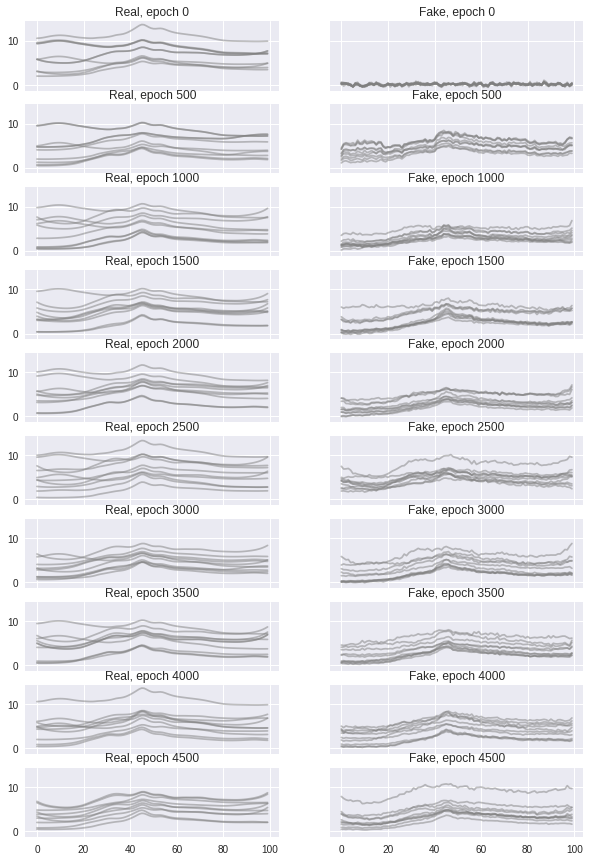
\includegraphics[width=17cm,height=15cm,keepaspectratio]{images/GAN_train.png}
\caption{Data generation process using GANs}
\label{fig:GANs train augmentation}
\end{center}
\end{figure}


\chapter{Deep learning model without augmentation}
\begin{figure}[ht]
	\begin{center}
		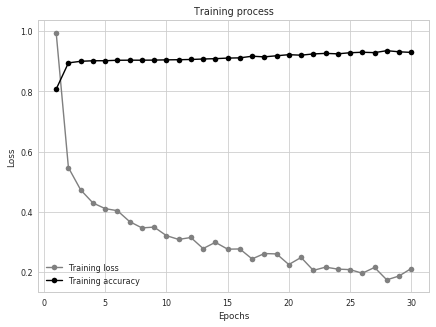
\includegraphics[width=12cm,height=10cm,keepaspectratio]{images/model1_training.png}
		\caption{Deep learning model without augmentation training process}
		\label{fig:first model training}
	\end{center}
\end{figure}

\chapter{Deep learning model training}
\begin{figure}[ht]
	\begin{center}
		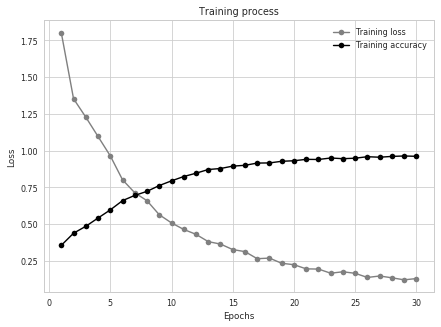
\includegraphics[width=\textwidth]{images/model_2.png}
		\caption{Training loss and accuracy for model with augmentation usign data-warping}
		\label{fig:second model}
	\end{center}
\end{figure}

\chapter{Deep learning model training}
\begin{figure}[ht]
	\begin{center}
		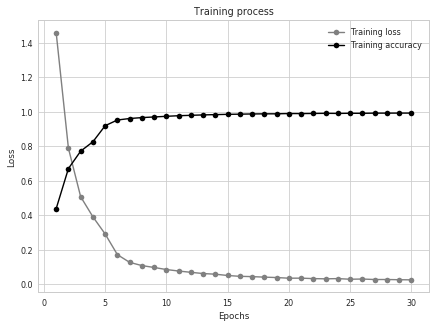
\includegraphics[width=\textwidth]{images/model_3.png}
		\caption{Training loss and accuracy for model with augmentation usign data-warping}
		\label{fig:third model}
	\end{center}
\end{figure}

\chapter{Model misclassification}
\begin{figure}[ht]
	\begin{center}
		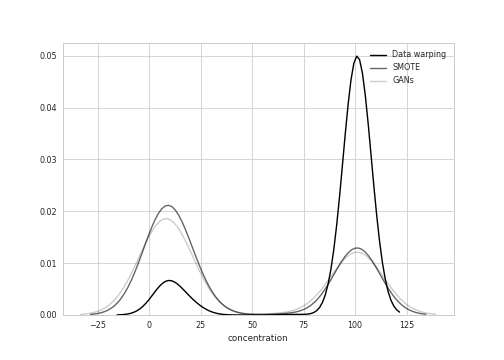
\includegraphics[width=\textwidth]{images/models_evaluation.png}
		\caption{Density plot of model missclassification at various concentration level }
		\label{fig:miss-classification}
	\end{center}
\end{figure}

% Load the bibliographic references
% ------------------------------------------------------------------
\startchapright
\phantomsection
\addcontentsline{toc}{chapter}{Bibliography}
% You can use several .bib files:
% \bibliography{thesis_sources,ietf_sources}
\bibliography{sources}

% End of document!
% ------------------------------------------------------------------
% The LastPage package automatically places a label on the last page.
% That works better than placing a label here manually, because the
% label might not go to the actual last page, if LaTeX needs to place
% floats (that is, figures, tables, and such) to the end of the 
% document.
\end{document}
\grid
